%\documentclass[twocolumn,showpacs,preprintnumbers,amsmath,amssymb]{revtex4}
\documentclass{report}
\usepackage{fancyhdr}
\usepackage{fullpage}
%\pagestyle{fancy}
%\fancyhead{}
\fancyfoot[L]{$ $Date: 2009-11-26 16:34:54 +0000 (Thu, 26 Nov 2009) $ $}
\fancyfoot[R]{$ $Revision: 1279 $ $}
\usepackage[small,labelfont=bf,textfont=it,width=0.9\textwidth]{caption} 
\usepackage{bm}

\renewcommand{\vec}{\bm}
\usepackage{graphicx}
\graphicspath{{../fig/}}
\usepackage{amssymb}
\usepackage{makeidx}
\makeindex 

 
\def\be{\begin{equation}}
\def\ee{\end{equation}}
\def\bee{\begin{eqnarray}}
\def\eee{\end{eqnarray}}
\def\l{{(0)}}
\def\f{{(1)}}
\def\minus{{\,\,\,\over \,\,\,}}
%
\def\black{\special     {ps: 0 0 0 setrgbcolor}}
\def\green{\special     {ps: 0 .5 0 setrgbcolor}}
\def\blue{\special      {ps: 0 0 1 setrgbcolor}}

%\def\black{}
%\def\blue{}
%\def\green{}

%\input{epsf}
%\newcommand{\epsfig}[3]{%
%    \begin{figure}[htbp]%
%        \begin{center}%
%            \setlength{\unitlength}{1.0cm}%
%            \begin{picture}(15,20)%
%                \epsfxsize=12cm%
%                \epsffile{#1}%
%                \end{picture}%
%            \end{center}%
%        \caption{#3}%
%        \{#2}%
%        \end{figure}%
% }


\title{GKW how and why}
\author{A.G. Peeters, D. Strintzi, Y. Camenen,\\
F.J. Casson, W.A. Hornsby, A.P. Snodin}
\date{Not maintained since CPC paper.  Please edit new version.}%\\
%\url{http://go.warwick.ac.uk/gkw}

\begin{document}

\def\compset#1{\vskip 0.2 truecm \noindent {\texttt #1 \hfill} \vskip0.2 truecm \noindent}

\pagenumbering{roman}
\maketitle
\cleardoublepage 
\centerline{\bf PREFACE} 
\vskip 1 truecm 

This \blue documentation \black comes with the GKW code. This code is distributed with the hope that 
it is useful, but the authors take no responsibility for it what so ever. 

There are several rules that apply to the use of this code 
\begin{itemize} 

\item You are not allowed to change the name of the code under any circumstances, even 
if you use part of the code no matter how small. This also applies if you make large 
changes to the code or even if you completely rewrite it. Add ons to the name, like 
$GKW\_GA$ are not allowed either. If you modify the code you should refer to it as 
'a modified version of GKW'. You are encouraged to write what the modifications include 
or cite a paper where it is spelled out. 

\item When GKW is used to produce results for a paper, you are obliged to cite the 
following references \hfill \break 
[1] A.G. Peeters, D. Strintzi, Phys. Plasmas, 11, 3748 (2004) \hfill \break
[2] A.G. Peeters, D. Strintzi, ...\hfill \break %PRL 2007?
[3] A.G. Peeters, Y. Camenen, F.J. Casson, W.A. Hornsby, A.P. Snodin, D. Strintzi, Computer Physics Communications, (2009) ...\hfill \break

The first is the original LINART code from which GKW was developed. In the second 
the code was used for the first time with major upgrades (kinetic electrons for instance) 
and the third is a general description of the code. We may change one of these citations
in the future. We promise to limit ourselves to 3 citations though (which should not stop 
you from citing any of our other excellent papers)  

\end{itemize} 

\noindent 
The restrictions above do not apply if the leading author (A.G.Peeters) gives explicit 
permission (He is unlikely to do so though).
The tone above is rather harsh, but you must realize that you can: 

\begin{itemize} 

\item Freely use the code for your own research purposes. You do not have to check with 
us or tell us what you are doing. (you are encouraged to do so, since we might be able 
to help you, and you might be able to help us) 

\item Publish as many papers as you like without telling us.

\item Make as many changes as you want to the source without any restrictions or 
obligation to share the changes (again you are encouraged to send us the modifications 
you have made, since it will help to further develop the code.

\item Read in the manual what the code does and how it does it.

\item Read in the manual what are the restrictions on the physics model.

\end{itemize} 



\cleardoublepage 

\tableofcontents
\cleardoublepage

\pagenumbering{arabic}

\vfill \eject 
\hbox to 2 truecm{\hfill}
\vskip 8 truecm 

\centerline{\selectfont \Huge I AM A USER} 
\addcontentsline{toc}{chapter}{I AM A USER}

\vfill  \eject 

\chapter{I want to do a run} 

Before you do any run it is important to realize that it is not all that hard to produce nonsense. 
The code is not under all conditions stable, and it is not always immediately obvious if a 
result is wrong. It is therefore important to diagnose your runs to make sure they are o.k.. 
It is your responsibility as a user to produce physically meaningful results. %See the section 'diagnose a run' to see what possibilities there are, and what to do if your run did not turn out quite the way you hoped it would.  

\section{Controlling the code} %Added by FC March 2008, updated Nov 2008
\index{input file}
\index{namelists}
To run GKW you must provide an input file \texttt{input.dat}. Provided with the code is a \texttt{input.dat.sample} file which describes all the possible input variables.  The \texttt{input.dat.minimum} file shows the variables that must be provided.  Many of the input switches are optional and default values will be used if they are not provided.  There are also other example input files provided.  The input variables are provided in fortran namelists, for example the namelist `control' contains the main switches for the code. The namelist examples presented in this chapter provide you with a basic set needed to run the code.  The namelists are sensitive to bad formatting or typos, in which case the code should infrom you which namelist has the problem.  

GKW tries to catch as many invalid input combinations as possible but there are probably many it can miss.  Most of the time if you input a set of incompatible switches the code will tell you and abort if necessary. For more minor errors the code will generate a warning that it is ignoring an input parameter and continue.  The actual input parameters the code runs with are written to input.out.  By renaming input.out to input.dat the code should run without the warnings.



\begin{footnotesize} \begin{verbatim}
&CONTROL
 NON_LINEAR = .false.      !Include the non linear terms, computationally expensive fft
 zonal_adiabatic = .false.,!If zonal flows corrections included for adiabiatic electrons
 order_of_the_scheme = 'fourth_order'	!or "second_order" in space		
 METHOD = 'EXP',        !Time integration "EXP" for explicit, "IMP" for implicit
 METH   = 2,            !Choice of algorithm for METHOD
 DTIM   = 0.02             !Time step size (normalized)
 NTIME  = 25,              !Number of iterations of NAVERAGE.
 NAVERAGE = 100,        !No of timesteps between re-normalisation, data output
 nlapar = .false.,      !true = keep the electromagnetic potential. false = electrostatic 
 collisions = .false.   !Turn on the collision operator
 disp_par = 1.0	        !Dissipation coefficient for parallel derivatives.
 disp_vp  = 0.0	        !Dissipation coefficient for parallel velocity space
 max_sec = 1000.        !Internal program kill time.
/
&GRIDSIZE
 NX = 83,        !Number of radial wave vectors - needs to be an odd number for fft
 N_s_grid = 50,  !Number of grid points along the field line 
 NPERIOD = 1,    !Integer - the field line makes 2*nperiod - 1 poloidal turns. 
 N_mu_grid   = 8,        !Number of magnetic moment grid points
 N_vpar_grid = 32,       !Number of grid points for parallel velocity 
 NMOD = 21,              !Number of binormal modes
 number_of_species = 1 	 !Number of kinetic species. 
/
\end{verbatim}\end{footnotesize}


\subsection{Timestep}
The timestep required for stability can vary greatly depending on input parameters or choice of scheme.  In particular kinetic electrons require a timestep $10^{-2}$ smaller.  Keeping the electromagnetic corrections for nonlinear runs is stabilising for low $\beta$ and can allow the timestep to be three times larger.  Clearly you should check the convergence of your results.

\subsection{Solver Methods}
The scheme can be either second order or fourth order in space.  The code has a choice of time integrator methods which can be used in the core solver as chosen by the input variable \texttt{METHOD}. The options are implicit (IMP) and explicit (EXP).  Within each method is a choice of algorithms chosen by the input variable \texttt{METH}. Currently the only safe options are:

\begin{itemize}
\item (METHOD, METH) = ('EXP', 1) Explicit - Modified mid point.
\item (METHOD, METH) = ('EXP', 2) Explicit - 4th order Runge Kutta.(RECOMMENDED)
\item (METHOD, METH) = ('EXP', 3) Explicit - 3rd order scheme.
\end{itemize}

The performance and stability of the different options varies and require careful usage.  Non linear runs can recalculate the time step size based on the Courant condition for numerical stability for the 4th order RK method.

\subsection{Parallelization}
\index{parallelization}
The code will parallelize first over the $\mu$ grid and (non-adiabatic) species, and then over the $v_{\parallel}$ and $s$ grid points.  The code will select what it considers to be the most appropriate parallelization given your input (this can be overridden by setting \texttt{N\_procs\_[sp|mu|vpar|s]} in the gridsize namelist).  Nevertheless it is sensible to have in mind a parallelization setup when you set the gridsize, as the user controls the number of processors the code will be run on and should choose a number that fits with the gridsize.

\subsection{Modes}
The spacing and location of the modes is determined by the `mode' namelist but is not immediately intuitive how this works.  

For \texttt{mode\_box=.false.} there is only the zero radial mode. The toridal modes are determined by the input list \texttt{kthrho} . For {mode\_box=.false.} the toroidal modes are input as a list i.e. \texttt{kthrho=0.1,0.2,0.3} (The \texttt{krhomax} is ignored), and the radial mode is not coupled at the end of the field line.

For \texttt{mode\_box=.true.}, the field line has one poloidal turn \texttt{nperiod=1}, and the radial modes are coupled at the end of the field line according to the ballooning shift due to the magnetic shear.  The torodial modes will be equally spaced $k_\theta\rho =0$ to \texttt{krhomax} (The \texttt{kthrho} input is ignored).  See \ref{ikxspace} for further details (the integer $p$ described there is input into the code as \texttt{ikxspace}).  The spreadsheet \texttt{modebox\_calculator} enables quick testing of the relevant quantities without running the code.

\begin{footnotesize}\begin{verbatim}
&MODE
 KTHRHO  = 0.5,1.0,  !Poloidal wave vector(s) if mode_box=.false.
 mode_box = .false., !Determines if there is a 2D grid of ky,kx. if true use nperiod = 1
                     !Also determines if kx modes are coupled at end of field line
 krhomax = 1.0,      !For mode_box, the maximum k_theta rho_i (ky) used
                     !Evaluated on the low field side of the outboard midplane
 ikxspace = 7,       !Determines spacing between kx modes (radial resolution against radial box size)
\end{verbatim}\end{footnotesize}

\begin{table}[h!]
\begin{center}
\begin{tabular}{ccccc}
 NS & ikxspace & NX & NPERIOD & mode\_box \\
\hline
 80      &    N/A   &  1  &    3    & false    \\
 16      &     1    &  5  &    1    & true     \\ 
\hline
 $n_s.(2n_p-1)$ &    N/A   &  1  &    $n_p$    & false    \\
 $n_s$    &     1    & $2n_p-1$ &  1   & true   \\

\end{tabular}
\caption{Equivalent formulations example with \texttt{mode\_box} true and false}
\end{center}
\end{table}

\subsubsection{Generating a linear growth rate spectrum}
GKW currently outputs the global growth rate in \texttt{time.dat} so the easiest way to generate a growth rate spectrum is do a batch of linear runs with \texttt{NMOD=1} and take the growth rate from each. If \texttt{mode\_box=.true.} and you have mode than one raidial mode, scan over \texttt{krhomax} to set the toroidal wavevectors (to keep the kx spacing the same you also have to vary ikxspace with krhomax); otherwise with {mode\_box=.false.} and \texttt{nx=1}, scan over \texttt{kthrho}.  The matlab scripts \texttt{create\_gkwscan} and \texttt{growth\_rate\_spec} help with creating the input and plotting the output; script \texttt{gkwnlin} runs the batch jobs. 

\subsection{Species}
There is no default species data, hence you must provide some. The species you input must satisfy quasi-neutrality. This requires you to set ratios of densities and charge appropriately.  You can input multiple ion species but only one negatively charged species is allowed.  Note that the number of species read in is controlled by the number of species parameter in the `gridsize' namelist and hence it is possible that later species data you specify will not be read in if this is set incorrectly.  The \texttt{number\_of\_species} input variable does not include adiabatic electrons but the species data for these will still be read if this the case.

\begin{footnotesize}
\begin{verbatim}
 &SPCGENERAL
  beta = 0.000,                !Plasma beta (not used if nlapar = .false.)
  adiabatic_electrons = .true. !kinetic electrons require a smaller timestep
 /
 &SPECIES
  MASS  = 1.0,  !Species mass in terms of reference mass
  Z     = 1.0,  !Species charge. If negative, assumed to be the electrons.
  TEMP  = 1.,   !Temperature of species scaled by reference temperature 
  DENS  = 1.,   !Density of species scaled by reference density 
  rlt   = 8,    !Temperature gradient R/LT
  rln   = 3.5,  !Density gradient R/Ln
  uprim = 0.0,  !Gradient of the toroidal rotation R^2 grad Omega / v_thref
 / 
 &SPECIES 
  MASS  = 2.72e-4,  !Electrons
  Z     = -1.0,     !Only one negatively charged species is allowed.
  TEMP  = 1.0, 
  dens  = 1.0,
  rlt   = 7.9,
  rln   = 3.5, 
  uprim = 0.0,
 /
\end{verbatim}
\end{footnotesize}

\section{Geometry} 
GKW is written in general coordinates so that in principle the code can deal with any toroidally symmetric 
equilibrium. This means that all the equations are expressed with the use of general tensors, and 
the metric elements. Currently the geometry dependent quantities are calculated in the code only for the $\hat s - \alpha$ equilibrium.  In addition, GKW can read CHEASE \cite{LUT96} output for
arbitrary flux
surface configurations. CHEASE takes an input of the shape of the last closed flux surface, a pressure gradient profile (and a boundary pressure), and a current profile. From these inputs, CHEASE
solves the Grad-Shafranov equation to find an equilibria flux surface configurations which it outputs as the poloidal flux. See the documentation file \texttt{gkwandchease.tex} for more information.

The simplest geometry is the 
$\hat s -\alpha$ geometry which consists of circular flux surfaces which are shifted with respect to 
each other by a magnitude determined by $\alpha$ which is the MHD parameter 
\be 
\alpha = -q^2R{d\beta \over dr}
\ee
\blue (As currently implemented in the code $\alpha = 0$).\black

The only other parameters that determine this equilibrium is the minor radius $r$ of the flux surface,
the safety factor $q$, and the magnetic shear $\hat s$. The minor radius is expressed in terms of the inverse 
aspect ratio $\epsilon$ 
\be 
\epsilon = {r \over R_{\rm ref}}  = {\tt eps}
\ee
where the reference major radius ($R_{\rm ref}$) is taken to be the major radius of the center of the
flux surface. 
In the equation above the name of the input variable is given in typewriter font. 
The shear follows from  
\be 
\hat s = {r \over q} {{\rm d} q \over {\rm d} r}  = {\tt shat} 
\ee
These parameters must be entered in the input file (which is always called input.dat) in the namelist 
called `geom'.

\begin{footnotesize}\begin{verbatim}
&GEOM
 shat = 1.0,
 q    = 2.0,
 eps  = 0.1
 /
&ROTATION
 VCOR = 0.0	!Rotation of the plasma vcor = Vtor / vthref = R Omega / vthref
 /
\end{verbatim} 
\end{footnotesize}

\section{Comparison with other codes} %Added Nov 2008 by FC
If you are trying to use GKW to compare to a result of another code, then you must understand the correspondance between the normalizations.  For many codes the thermal velocity is normalized differently and hence GKW's $k_{\theta}\rho_i$ may be a factor of $\sqrt{2}$ larger.  Note also that \texttt{rlt} in the input file is the value of $R/L_T$ and \texttt{rln} is $R/L_n$.

Here we outline how to compare GKW results with codes that use gyro-Bohm units.
In the case where $T_e=T_{\rm ref}$ and $m_i=m_{\rm ref}$ the sound speed $c_s=\sqrt{T_e / m_i}$
converts to the GKW reference velocity as $v_{\rm thref}=\sqrt{2} c_s$ and the gyro-Bohm Larmor
radius $\rho_s=c_s/\Omega_{ci}$ is related to the GKW reference Larmor radius by $\rho_s=\rho_{\rm
ref}/\sqrt{2}$. For full details see section \ref{normalization}.

Hence the GKW time normalization may be converted:
\begin{equation}
t_N = {v_{\rm thref} \over R} t = \sqrt{2}{c_s \over R} = \sqrt{2} \left({a \over R}\right) \left({c_s \over a}\right) t
\end{equation}
This time normalization is used in all GKW output of times and rates and this must be accounted for when comparing results with other codes.  %Also set B_N to 1 ????

The fluxes diagnostic outputs the heat fluxes ${\texttt eflux} = q_i^N$ which may be converted to a heat diffusivity
\begin{equation}
\chi_i^N={q_i^N \over R/L_T}={R \over \rho_{\rm ref}^2 v_{\rm thref}} \chi_i = {1 \over 2\sqrt{2}}\left({R \over a}\right)\left({a \over \rho_s^2 c_s}\right) \chi_i 
\end{equation}
The particle and momentum fluxes can be converted similarily.  For further details see section \ref{fluxes}.

%\section{Setting up a run and initial checks}
%
%For linear runs should have symmetric in s.  Stable should have a smooth solution in s
%Check convergence of growth rates and fluxes ratios



%For kinetic runs need kxmax 3*kymax.  Expect ion fluxes 3 x bigger than for adiabatic and 3 x bigger that electron fluxes
%For nonlinear runs check fluxes saturate, want range in fluxes <80% - use minimum dissipation that gives this.
%For kinetic runs use nlapar=.true. and beta 3e-4 with timestep 0.003
%Use an odd number for n_s_grid if you want a point in the middle of the field line (but for parallelisation in s should still have some factors!)
%Choose ikxspace to choose get balance between x resolution and box size - usually aiming for a square box and kxmax = 3x krhomax (in rho ref units)
%Check the parallel output - should be not too noisy for stable runs.
%Check the ky spectrum is well covered by the modes
%Check the linear growth rate spectrum is well covered by the modes.
%Nonlinear: check the timestep didn't collapse.
%suitable dissipation coeffcients.  
%guidline suitable (minimum and not necessirly well converged!) grid sizes for kinetic ITG / TEM cases. nmod=21, nx=167, krhomax=1.41, ikxspace=6, ns=16, nvpar=32, nmu=8, dtim=0.003, disp_par=disp_vp=1.5
%particle fluxes should be zero for a single species, should be same for two species
%time averaged momentum flux should be zero for no s-alpha, no shear, no uprime.

\cleardoublepage 

%\pagenumbering{arabic}

\vfill \eject 
\hbox to 2 truecm{\hfill}
\vskip 8 truecm 

\centerline{\selectfont \Huge I AM A PHYSICIST} 
\vskip 8 truecm 
\blue Read this section alongside the CPC paper which may have some corrections.\black
\addcontentsline{toc}{chapter}{I AM A PHYSICIST}

\vfill  \eject 

\chapter{Geometry}

\section{Field aligned Hamada coordinates} 
\index{coordinates, flux tube}

In this chapter we will work out the coordinates attached to the magnetic field geometry. 
Several functions will be defined that are used in the gyro-kinetic equation. The 
development of the material in this section has benefited a lot from the write-ups 
of Dr. B.D. Scott \cite{Scott}

We start with an arbitrarily shaped, but toroidally symmetric geometry. We assume that 
we have a semi-orthogonal coordinate system $(\psi,\theta,\phi)$, where $\psi$ is the 'radial'
coordinate (i.e. ${\bf B}\cdot \nabla \psi = 0$), $\theta$ is the poloidal angle (upward 
on the outboard midplane), and $\phi$ is the toroidal angle (clockwise when viewed from 
above). Furthermore, we will assume that the magnetic field and quantities like the major 
radius are known in this coordinate system. Below we go through two coordinate transformations. 
The first will make the field lines straight in the new coordinates, and the second will 
align one of the coordinates with the magnetic field. 

In the first step we transform the poloidal and toroidal angle 
\be 
s = s(\psi,\theta), \qquad \gamma = \gamma(\psi,\theta,\phi)
\ee 
in such a way that the contra-variant components of the magnetic field are flux functions 
in the new coordinate system ($B^s = B^s(\psi)$, $B^\gamma = B^\gamma(\psi)$). These 
coordinates are known as Hamada coordinates \cite{HAM62}\index{Geometry:Hamada coordinates}. 
Note that the new coordinate $\gamma$ is still an ignorable coordinate, since any function that is independent of $\phi$
will be independent of $\gamma$ ($f(\theta,\psi) \rightarrow f(s,\psi)$) after the coordinate 
transformation. The transformation of the poloidal angle is chosen such that $B^s$ becomes 
a flux function 
\be 
B^s = {\bf B} \cdot \nabla s = {\bf B}\cdot \nabla \theta {\partial s \over \partial \theta} 
+ {\bf B} \cdot \nabla \psi {\partial s \over \partial \psi} = {\bf B} \cdot \nabla \theta 
{\partial s \over \partial \theta}
\ee 
From which the relation between $s$ and $\theta$ can be derived 
\be
{\partial s \over \partial \theta}={B^{s} \over {\bf B \cdot \nabla \theta}}\Leftrightarrow
\int_{0}^{\theta}{\partial s \over \partial \theta}d\theta =s=B^{s}\int_{0}^{\theta}{d\theta \over 
{\bf B}\cdot \nabla \theta}
\ee
since $B^{s}$ does not depend on $\theta$ (flux function) and
\be
\oint {\partial s \over \partial \theta}d\theta =1=B^{s}\oint {d\theta \over {\bf B}\cdot \nabla 
\theta}\Leftrightarrow B^{s}={1 \over \oint {d\theta \over {\bf B}\cdot \nabla \theta} }
\ee
which gives the following equation for s:
\be 
s(\theta,\psi) = {\int_0^\theta {{\rm d} \theta^\prime \over {\bf B} \cdot \nabla \theta^\prime} 
\biggl /  \oint {{\rm d}\theta^\prime \over {\bf B}\cdot \nabla \theta^\prime}} \qquad 
{\rm with} \qquad 
B^s =  {1
\biggl /  \oint {{\rm d}\theta^\prime \over {\bf B}\cdot \nabla \theta^\prime}}
\ee  
where the normalizing constant has been chosen such that the domain [-1/2,1/2] in $s$ corresponds 
to one poloidal turn. 

The new coordinate is closely related to the flux surface average. This average is defined 
as the volume average between two flux surfaces in the limiting case in which the distance between 
the flux functions goes to zero. One can derive the following relation  
\be 
\langle g \rangle = \oint {{\rm d} l_p \over B_p } g \biggl / \oint {{\rm d} l_p \over B_p }
\ee
where $l_p$ is the length in the poloidal direction (${\rm d}l_p = \vert {\bf e}_\theta \vert 
{\rm d} \theta$), $B_p$ is the poloidal component of the magnetic field strength ($B_p = 
{\bf B}\cdot \nabla \theta / \vert \nabla \theta \vert$), and the integral is to be taken at 
constant $\psi$. Inserting the expressions for the 
poloidal length and the poloidal magnetic field strength and using $\vert {\bf e}_\theta\vert 
\vert \nabla \theta \vert = 1$ one obtains 
\be 
\langle g \rangle = \oint {\rm d}s g 
\ee 


For the transformation of the toroidal angle we choose 
\be 
\gamma = {\phi \over 2 \pi} + g(\theta,\psi) 
\ee
The $2\pi$ is added here such the domain [0,1] in $\gamma$ will correspond to one toroidal 
turn around the flux surface. The contra-variant component of the magnetic field is 
\be 
B^\gamma = {F \over 2\pi} {1\over R^2} + {\bf B} \cdot \nabla \theta {\partial g \over \partial 
\theta} 
\ee 
where $F = R B_t = F(\psi)$ is a flux function. (Here $B_t$ is the toroidal magnetic field 
strength $B_t = {\bf B} \cdot \nabla \phi / \vert \nabla \phi \vert$ where $\vert \nabla \phi 
\vert = 1/R$ with $R$ being the local major radius)
From the expression above one can derive 
\be 
g(\theta,\psi) = \int_0^\theta {{\rm d}\theta^\prime \over {\bf B}\cdot \nabla \theta^\prime } 
\biggl [ B^\gamma - {F \over 2\pi} {1 \over R^2} \biggr ] 
\ee 
Demanding that $g$ is periodic
\be
\oint {{\rm d}\theta^\prime \over {\bf B}\cdot 
\nabla \theta^\prime } 
\biggl [ B^\gamma - {F \over 2\pi} {1 \over R^2} \biggr ] =0
\ee
yields 
\be 
B^\gamma = {F\over 2 \pi } \biggl \langle {1\over R^2} \biggr \rangle 
\ee 
The coordinate $\gamma$ can then be expressed as 
\be 
\gamma = {\phi \over 2\pi} + {F \over 2\pi} \int_0^\theta {{\rm d} \theta^\prime \over {\bf B}
\cdot \nabla \theta^\prime} \biggl [ \biggl \langle {1\over R^2} \biggr \rangle - {1\over R^2} 
\biggr ] 
\ee 
The coordinates $(\psi,s,\gamma)$ are the Hamada coordinates. The expression above should 
allow these coordinates to be calculated for an arbitrary toroidally symmetric geometry. 

We now go through the second coordinate transformation where one of the coordinates is 
aligned with the magnetic field, i.e. we demand 
\be 
{\bf B} \cdot \nabla = B^s {\partial \over \partial s}
\ee
Note that this does not mean that $\nabla s$ is in the direction of the magnetic field. 
In general it is not. The transformation is 
\be 
\zeta = \zeta(s,\gamma,\psi) 
\ee
In the new coordinates 
\be
{\bf B}\cdot \nabla =B^{\psi}{\partial \over \partial \psi}+B^{s}{\partial \over \partial s}+
B^{\zeta}{\partial \over \partial \zeta}
\ee
where $B^\psi$ is zero. The transformation to field aligned coordinates is the transformation 
for which $B^\zeta = 0$. The latter condition can be formulated as 
\be 
B^\gamma {\partial \zeta \over \partial \gamma} + B^s {\partial \zeta \over \partial s} = 0
\ee 
which is satisfied for the simple linear transformation
\be 
\zeta =  q s - \gamma \qquad {\rm where} \qquad q = {B^\gamma \over B^s} 
\ee
From the field line equation it follows that 
\be 
{{\rm d} \gamma \over {\rm d} s} = {B^\gamma \over B^s} \qquad \rightarrow \qquad 
\oint {{\rm d} \gamma \over {\rm d} s} {\rm d} s = \oint {B^\gamma \over B^s} {\rm d} s = q 
\ee 
i.e. $q = q(\psi)$ is indeed the safety factor. 

Note that the coordinate transformation above flips the sign of the toroidal angle. 
The right handed coordinate system can therefore be defined as $(\psi,\zeta,s)$. 
The Jacobian of the new coordinate system can be expressed in terms of the original 
Jacobian through 
\be 
(\nabla \psi \times \nabla \zeta) \cdot \nabla s = {1 \over J_{\psi  \zeta s} } = 
{1\over 2 \pi}{\partial s \over \partial \theta} {1 \over J_{\psi \theta \phi}} 
\ee 
From which it follows 
\be 
J_{\psi  \zeta s} = 2\pi {\bf B} \cdot \nabla \theta \oint {{\rm d} \theta^\prime \over 
{{\bf B} \cdot \nabla \theta^\prime}} J_{\psi \theta \phi} 
\ee 



We note here that the coordinates $s$ and $\zeta$ are dimensionless, but that the 
dimension of $\psi$ is not yet defined. We will always use a normalized $\psi$ that 
is dimensionless (see \ref{normalization} for a discussion on the normalization) 

\section{Metric elements} 
%Some updates to this section in the CPC paper, check for consistency here.
\section{Short look ahead} 
\index{geometry tensors}
So far we have introduced the coordinates. Of course, to solve the gyro-kinetic 
equation we will have to calculate some specific quantities in the general 
coordinate system. In the next chapter these will be introduced. To proceed 
with the discussion of the geometry we define them here 
\be 
{\cal F} = {R_{\rm ref} B^s \over B} \qquad \rightarrow \qquad 
R_{\rm ref} {\bf b} \cdot \nabla  = {{\cal F}} {\partial \over \partial s} 
\ee
\be 
{\cal D}^\alpha = {R_{\rm ref}^2 {\bf B} \times \nabla B \over B^2 B_N} \cdot \nabla x_\alpha 
\ee 
\be 
{\cal E}^{\alpha \beta} = {R_{\rm ref}^2\over 2 B_N} (\nabla x_\alpha \times \nabla x_\beta) \cdot {\bf b} 
\ee 
\be 
{\cal G} = {R_{\rm ref} {\bf B } \cdot \nabla B \over B^2} %%={\cal F} {\partial ln B \over \partial s} ??
\ee
\be 
{\cal H}^\alpha = {R_{\rm ref}^2 \over v_{\rm thref}}{\bf \Omega}_\perp \cdot \nabla x_\alpha 
\ee
\be 
{\cal I}^\alpha = {R_{\rm ref}^2 \Omega^2 \over 2 v_{\rm thref}^2 B_N } (\nabla x_\alpha \times \nabla R^2) 
\cdot {\bf b} 
\ee
In these equations $R_{\rm ref}$ is the reference value of the major radius, i.e. it is 
simply a normalizing constant. $B_N$ is the magnetic field normalized to a reference value 
$B_{\rm ref}$, $v_{\rm thref}$ is a reference (thermal) velocity, and $\Omega$ is the angular 
(toroidal) rotation frequency of the plasma. In the next sections these coefficients will be 
worked out for different geometries.  Note that for benchmarking against other gyrokinetic codes the $B_{N}$ may need to be approximated to 1. \blue You should check your version of the code in the
geom module, as this  may have been done. \black
Note that the sign convention is $\Omega>0$ for a plasma flowing in the direction of $\mathbf{B}$, which  means that $\mathbf{\Omega}=-\Omega\mathbf{\nabla}Z$ for $\mathbf{B}\cdot\mathbf{\nabla \phi}>0$ and $\mathbf{\Omega}=\Omega\mathbf{\nabla}Z$ for $\mathbf{B}\cdot\mathbf{\nabla \phi}<0$.


\section{$s-\alpha$ geometry} 
\index{$s-\alpha$}
The simplest choice of the geometry is the $s-\alpha$ model. This model assumes circular 
flux surfaces which can be shifted with respect to each other. The inverse aspect rato $\epsilon = r / R$ 
is assumed small, with $R=R_{\rm ref}$, and only the lowest order in an $\epsilon$ expansion is kept. 
The poloidal magnetic field is assumed much smaller than the toroidal magnetic field
\be 
B \approx |B_t| \qquad 
q \approx s_{\rm B}s_{\rm j} {r |B_t| \over R |B_p|} 
\ee 
where the signs of the magnetic field ${\bf B}$ and current density ${\bf j}$ are defined as $s_{\rm B}=\textrm{sign}(\bf{B}\cdot\nabla\phi)$ and $s_{\rm j}=\textrm{sign}(\bf{j}\cdot\nabla\phi)$
with $\phi$ increasing clockwise when the torus is viewed from above. 
The coordinates can be approximated as 
\be 
\psi = {r \over R}, \qquad 
\zeta =  {1\over 2 \pi} [q \theta - \phi ] \qquad 
s = {\theta \over 2 \pi }  \qquad 
\ee
The gradients are approximated as  
\be 
\nabla \psi = {1\over R} {\bf e}_r \qquad 
\nabla \zeta = {s_{\rm B}s_{\rm j}|q| \over 2 \pi r} [ {\bf e}_\theta + \hat s \theta {\bf e}_r ]  \qquad 
\nabla s = {1 \over 2 \pi r} {\bf e}_\theta
\ee 
Note that the gradient of the toroidal angle is ordered small compared with the gradient of the poloidal
angle (times q) and is neglected in the gradient of $\zeta$. The contravariant components of the 
magnetic field are 
\be 
B^s = s_{\rm j}{|B_p| \over 2 \pi r} \qquad 
B^\zeta = -{s_{\rm B}|B_t| \over 2 \pi R}  
\ee 
The gradient of the magnetic field strength is assumed to be in the direction of $\nabla R$ and the 
drift term is approximated as 
\be 
{\bf B} \times \nabla B = -s_{\rm B}{B^2 \over R} [ \cos \theta {\bf e}_\theta + \sin \theta {\bf e}_r ] 
\ee 


With this expression one can evaluate the quantities needed for the numerical computations 
\be 
{\cal F} = {s_{\rm j}\over 2 \pi |q|} 
\ee
\be 
{\cal D^\psi} = - {s_{\rm B}\over B_N} \sin (2 \pi s)
\ee 
\be 
{\cal D}^\zeta = - {s_{\rm j}|q| \over 2 \pi \epsilon B_N} [ \cos (2 \pi s) + 2 \pi \hat s s \sin (2 \pi s) ] 
\ee
\be 
{\cal D}^s = -{s_{\rm B}\over 2 \pi \epsilon B_N} \cos ( 2 \pi s) 
\ee
\be 
{\cal G} =  {s_{\rm j}\epsilon \over |q|} \sin ( 2 \pi s) 
\ee
\be 
{\cal E}^{\psi \zeta} = {s_{\rm j}|q| \over 4 \pi \epsilon B_N}
\ee
\be 
{\cal E}^{\psi s} =  {s_{\rm B} \over 4 \pi \epsilon B_N}
\ee
\be 
{\cal E}^{\zeta s} =  { s_{\rm j}|q| \over 4 \pi \epsilon^2 B_N } \hat s s 
\ee
Finally 
\be 
R^2g^{\zeta \zeta} = \biggl ( {q \over 2 \pi \epsilon} \biggr )^2 + \biggl ( {q \over\epsilon} \hat{s} s \biggr )^2 \qquad 
\ee
\be 
R_{\rm ref}^2 g^{\zeta \psi} = {s_{\rm B}s_{\rm j}|q| \over \epsilon} \hat s s 
\ee 
\be  
R_{\rm ref}^2 g^{\psi \psi} = 1 
\ee 
%{\cal E}^{\psi s} and {\cal D} not used in code, not included in CPC paper

\section{Shifted circular surface geometry} 


The shifted circular surface geometry is defined in the ($R,Z$) plane (using cylindrical coordinates
$(R,\phi,z)$. 
\be 
R = r \cos \theta + \Delta(r) + R_0 \qquad {\rm with} \qquad \Delta(0) = 0 
\ee
\be 
Z = r \sin \theta
\ee
Surfaces of constant $r$ are assumed to be flux surfaces. One can confusingly define two major 
radii. One is the radius of the magnetic axis $R_0$, and one is the major radius of the centre 
of the surface $R_c$ 
\be 
R_c = (R(\theta =0) + R(\theta = \pi) )/2 = R_0 + \Delta(r) 
\ee
Since the first one is a constant while $R_c$ depends on $r$, we will choose to normalize all 
the radii with $R_0$, i.e. 
\be 
R_{\rm ref} = R_0
\ee
The normalized radial coordinate then is 
\be 
\psi = r / R_0 = \epsilon
\ee
and we will define a normalized major radius that gives the centre of the surface as 
\be 
R_{cN} = 1 + {\Delta (r) \over R_0} 
\ee

From the equations above one can work out
\be 
\biggl [ \matrix{ \nabla r \cr \nabla \theta} \biggr ]  = {1\over r (1 + \Delta^\prime \cos \theta)} 
\biggl [ \matrix{ r \cos \theta & r \sin \theta \cr - \sin \theta & \Delta^\prime + \cos \theta} 
\biggr ] \biggl [ \matrix{ \nabla R \cr \nabla Z } \biggr ] 
\ee
where 
\be 
\Delta^\prime = {{\rm d} \Delta \over {\rm d} r} 
\ee
The poloidal magnetic field can be written as 
\be 
{\bf B}_p = B_p {{\bf e}_\theta \over \vert {\bf e}_\theta \vert} \qquad 
{\bf e}_\theta = {\partial {\bf x} \over \partial \theta} = \biggl [ \matrix{-r \sin \theta \cr r \cos \theta}
\biggr ]  
\ee 
From which it folows that 
\be 
{\bf e}_\theta \cdot \nabla \theta = 1 \qquad {\bf B} \cdot \nabla \theta = B_p / r 
\ee 
From flux conservation 
\be 
R B_p {\rm d}l_\perp = {R B_p \over \vert \nabla r \vert } {\rm d} r = {\rm constant} 
\ee
It follows that  
\be 
{B_p \over B_p(\pi/2)} = {R_{cN}(\psi) \over (1 + \Delta^\prime(\psi) \cos \theta) (R_{cN}(\psi) + \psi \cos \theta)}
\ee
The integral to obtain $s$ and $B^s$ can be easily performed 
\be 
B^s = {B_p(\pi/2)\over 2 \pi ( 1 + \psi \Delta^\prime / 2 R_{Nc} )}
\ee
\be 
s = {\theta \over 2 \pi} + {2 \psi \sin \theta + 2 \Delta^\prime R_{cn} \sin \theta + \Delta^\prime \psi 
\cos \theta \sin \theta \over 4 \pi R_{cn} ( 1 + \Delta^\prime \psi / 2 R_{cn})}
\ee
After some manipulations also the flux surface average of $1/R^2$ can be expressed as 
\be 
\biggl \langle {1 \over R^2} \biggr \rangle = {1\over R_0^2} {1 \over R_{cN} + \psi \Delta^\prime / 2} 
\biggl [ {1 - \Delta^\prime \over \sqrt{R_{cN}^2 - \psi^2} } + {\Delta^\prime \over \psi} \biggr ] 
\ee


\section{General geometry}
The metric elements for general toroidal MHD equilibria can be obtained from the CHEASE code \cite{LUT96}. The sign of the magnetic field and plasma current are not taken into account into CHEASE
which always consider that ${\bf B}$ and ${\bf j}$ are in the direction opposite to $\nabla \phi$ (here
$\nabla \phi = \nabla \phi_{\rm GKW}$, as everywhere in this document). The sign of ${\bf B}$ and ${\bf j}$ are therefore specified in GKW, in the \texttt{GEOM} namelist
using the variables \texttt{SIGNB} and \texttt{SIGNJ} defined as in the previous section by $s_{\rm B}=\textrm{sign}(\bf{B}\cdot\nabla\phi)$ and $s_{\rm j}=\textrm{sign}(\bf{j}\cdot\nabla\phi)$. When
CHEASE is used, the absolute value of the safety factor and magnetic shear (used for the periodicity condition and to set the radial wave vector grid) is taken from the equilibrium reconstruction and
the values specified in the namelist \texttt{GEOM} are not read. The values of $\beta'$ is also calculated consistently with the equilibrium reconstruction.



\section{Summary of the sign conventions in GKW} 
\label{signs}
In GKW, the cylindrical coordinate system $(R,Z,\phi)$ is right handed, which means that $\phi$ is increasing clockwise when the torus is viewed from above.\\
The toroidal rotation is defined positive for a plasma flowing in the direction of ${\bf B}$.\\
The mode frequency is defined positive for a perturbation evolving in the direction opposite to $\nabla \zeta$. This corresponds to the ion $\nabla B$ drift direction if $s_{\rm j}=1$ and to the
electron $\nabla B$ drift direction if $s_{\rm j}=-1$.  See also Fig.~\ref{directions}\\
Coordinate system:
\begin{itemize}
 \item $\psi=\varepsilon=(R_{\rm max}-R_{\rm min})/(2R_{\rm ref})$ is always increasing from the plasma center to the plasma edge.
 \item $s$ is always increasing upwards from the low field side midplane. It is zero at the height of the magnetic axis, on the low field side midplane.
 \item $\zeta$ is always increasing in the direction opposite to $\phi$ (i.e. anticlockwise when viewed from above) at constant $\psi$ and $s$. The direction of $\nabla \zeta$ in the poloidal plane is
given by $\textrm{sign}(\nabla s \cdot \nabla \zeta)=\textrm{sign}(\nabla 
\zeta \cdot \nabla \theta)=s_{\rm B}s_{\rm j}$
\end{itemize}

\bee
\textrm{sign}({\bf B} \cdot \nabla \phi)&\equiv& s_B \\
\textrm{sign}({\bf j} \cdot \nabla \phi)&\equiv&s_j \\
\textrm{sign}({\bf B} \cdot \nabla \theta)&=& s_j \\
\textrm{sign}({\bf B} \cdot \nabla s)&=& s_j \\
\textrm{sign}(\nabla \phi \cdot \nabla \zeta)&=& -1 \\
\textrm{sign}(\nabla s \cdot \nabla \theta)&=& 1\\
\textrm{sign}(\nabla \theta \cdot \nabla \zeta)&=& s_B s_j \\
\textrm{sign}(B_\theta \nabla \theta \cdot \nabla \zeta)&=& s_B \\
\textrm{sign}(\nabla s \cdot \nabla \zeta)&=& s_B s_j \\
{\bf B} \cdot \nabla \zeta&=& 0 \\
{\bf \Omega} &=& -s_B \Omega \nabla z \\
u &=& R \Omega 
\eee
%The direction of zeta is flipped by both sign_j reversal and sign_B reversal.

\begin{thebibliography}{10}

\bibitem{Scott} B.D. Scott, private communications and web page 
www.rzg.mpg.de/~bds

\bibitem{HAM62} S. Hamada, Kakuyugo Kenkyu {\bf 1}, 542 (1958)  

\bibitem{LUT96} H. L\"utjens, A. Bondeson and O. Sauter, Comput. Phys. Commun.{\bf 97}, 219 (1996)

\end{thebibliography}

\chapter{The gyro-kinetic set of equations }

This chapter deals with the basic equations that  are solved in the code. 

\section{The gyro kinetic framework}

The starting point of the equation for the evolution of the distribution function is the 
gyro-kinetic theory formulated in Refs \cite{LIT83,HAH88,BRI88,SUG00}. In GKW these equations 
are solved up to first order in Larmor radius over the major radius ($\rho_*$), which 
is assume to be a small quantity. In order to determine which of the terms in the 
original formulation of the theory (which is accurate up to second order in $\rho_*$) 
must be kept, we will here briefly discuss the ordering.

A thermal velocity ($v_{\rm th}$) and a major radius ($R$) are used to normalize the length and 
time scales. For the gradients we assume 
\be 
R \nabla_\parallel  \approx 1 \qquad 
R \nabla_\perp \approx 1/ \rho_*
\ee 
i.e. the solution is assumed to have a length scale of the order of the system size along the 
field, but can have a structure of the order of the Larmor radius perpendicular to the 
magnetic field. This difference in length scales makes that we will evaluate the velocity 
along the field in lowest order only (i.e. of the order of $v_{\rm th}$), but have to go to 
first order (order $\rho_* v_{\rm th}$) for the perpendicular motion. Both the perturbations in 
the electro static potential $\phi$ as well as the vector potential are retained. For the 
latter it is, however, assumed that 
\be 
{\bf A} = A_\parallel {\bf b} 
\ee
i.e. no compressional effects are kept in the magnetic field evolution. 
Note that the vector potential above is the perturbed vector potential not to be confused 
with the one connected with the equilibrium magnetic field. 
The potential and the vector potential are taken to be of the order 
\be 
\phi \approx {T \over e} \rho_* \qquad 
A_\parallel \approx {T \over e v_{\rm th}} \rho_* , 
\ee
where $T$ is the temperature, and $e$ is the elementary charge.  
From this assumption it can be derived that the ${\bf E} \times {\bf B}$ velocity is of the order $\rho_* v_{\rm th}$, 
i.e. no higher order corrections must be kept. A similar argument applies to the tilting of 
the field line due to the perturbed vector potential. 

Gyro-center coordinates (${\bf X},\mu,v_\parallel$) are used, with ${\bf X}$ being the gyro
center position, $v_\parallel$ the parallel velocity, and $\mu$ the magnetic moment 
\be 
\mu = {m v_\perp^2 \over 2 B} 
\ee 
where $v_\perp$ is the velocity component perpendicular to the magnetic field ${\bf B}$, $m$
is the particle mass and $B$ is the magnetic field strength. The magnetic moment is an 
invariant of motion, but the parallel velocity changes due to the electric field acceleration 
and the mirror force. It turns out that for consistency one needs to keep both the lowest 
as well as the first order (in $\rho_*$) contribution to the acceleration. 

Finally, also the approximation known as $\delta f$ approximation will be made. This approximation
assumes that the perturbed distribution $f$ is much smaller than the background distribution 
$F$, but has a length scale of the order of the Larmor radius whereas the background varies 
on the length scale of the system size 
\be 
f \approx \rho_* F \qquad 
{\partial f \over \partial v_\parallel} \approx \rho_* {\partial F \over v_\parallel}  \qquad 
\nabla f \approx \nabla F 
\ee
These relations mean that what is known as the velocity non-linearity (combinations of the 
electromagnetic fields and the velocity space derivative of the perturbed distribution) can
neglected in the evolution equation for the perturbed distribution.  


With the help of these approximations the gyro-kinetic equation of Refs. \cite{LIT83,HAH88,BRI88,SUG00}
can be rewritten. Starting point is the Lagrangian \index{Lagrangian}
\be
\gamma=\left({e\over c}{\bf A}+{e\over c}A_{\parallel}{\bf b}+m{\bf v} \right)\cdot d{\bf x}-\left({m\over 2}v^{2}+e\phi \right)dt
\ee
The coordinates are transformed into guiding center coordinates. The electrostatic guiding center
Lagrangian in known, and can be found in Hahm 1988. For the magnetic perturbations we take that
\be
A_{\parallel}({\bf X}+{\bf \rho}){\bf b} \cdot d({\bf X}+\rho)
\ee
where $\rho =\rho({\bf X},{\mu},{\theta})$. All the derivatives of $\rho$ will give vectors
perpendicular to the magnetic field. Thus if there is not a perpendicular magnetic potential
perturbation, the only term that survives is
$$A_{\parallel}{\bf b}\cdot d{\bf X}$$
Then the guiding center Lagrangian is
\be
\gamma =\left({e\over c}{\bf A}+{e\over c}A_{\parallel}{\bf b}+mv_{\parallel}{\bf b} \right)\cdot 
d{\bf X}+\mu d\theta -\left({m\over 2}v_{\parallel}^{2}+\mu B+e\phi \right)dt
\ee
This Lagrangian is transformed in the gyrocenter coordinates with the Lie transforms.
To the first order, if there are no perpendicular perturbations in the magnetic potential,
we can just substitute the perturbations of the fields with the respective gyroaveraged quantities. 
This can also be derived rigorously with the Lie transforms. The new Lagrangian will be
\be
\Gamma =\left({e\over c}{\bf A}+{e\over c}<A_{\parallel}>{\bf b}+mv_{\parallel}{\bf b} \right)\cdot 
d{\bf X}+\mu d\theta -\left({m\over 2}v_{\parallel}^{2}+\mu B+e<\phi> \right)dt
\ee
where now ${\bf X},\mu,v_{\parallel},\theta$ are the gyrocenter coordinates. From this one can derive 
the equations of motion using the Euler Lagrange equations
\be
\omega_{ij}{dz^{j}\over dt}={\partial H \over \partial z^{i}}-{\partial \gamma_{i}\over \partial t}
\ee
where $H$ is the Hamiltonian and 
\be
\omega_{ij}={\partial \gamma_{j}\over \partial z^{i}}-{\partial \gamma_{i}\over \partial z^{j}}
\ee
are the Lagrange brackets.

The Lagrange brackets that are of interest are
\be
\omega_{X_{i}X_{j}}={e\over c}\epsilon_{ijk}{\hat B}_{k}
\ee
\be
\omega_{{\bf X}U}=-m{\bf b}
\ee
where 
\be
{\hat {\bf B}}=\nabla \times {\bf A}+\nabla \times A_{\parallel}{\bf b}+{mc \over e}v_{\parallel}\nabla \times {\bf b}
\ee

Choosing $i=U$ we get that
\be
m{\bf b}\cdot {\dot {\bf X}}=mv_{\parallel}
\ee
Choosing $i={\bf X}$ we get that
\be
m{\dot v}_{\parallel}{\bf b}-{e\over c}{\dot {\bf X}}\times {\hat{\bf B}}=-e\nabla <\phi>-\mu \nabla B-{e\over c}
{\partial <A_{\parallel}>\over \partial t}{\bf b}
\ee
and taking that
\be
{\bf E}=-\nabla \phi -{1\over c}{\partial <A_{\parallel}>\over \partial t}{\bf b}
\ee
we get that
\be
m{\dot v}_{\parallel}{\bf b}-{e\over c}{\dot {\bf X}}\times {\hat{\bf B}}=e{\bf E}-\mu \nabla B
\ee

We can cross this equation with ${\bf b}$ to derive the equation for $\dot X$. To derive the equation of GKW we have
to approximate
\be
\nabla \times (<A_{\parallel}>{\bf b})\approx \nabla  (<A_{\parallel}>)\times {\bf b}
\ee
Then the equation of $\dot X$ is.
\be 
{{\rm d} {\bf X} \over {\rm d} t} = v_\parallel {\bf b} + {\bf v}_D + {\bf v}_E + {\bf v}_{\delta B_\perp}, 
\ee
To derive the equation for $v_{\parallel}$ we dot with $\dot X$. This gives
\be
mv_{\parallel}{\dot v}_{\parallel}={\dot {\bf X}}\cdot \left(e{\bf E}-\mu \nabla B\right)
\ee


\section{Equation for the evolution of the distribution function} 

In the previous section the evolution equation for the guiding center motion and the parallel velocity 
were formulated 
\be 
{{\rm d} {\bf X} \over {\rm d} t} = v_\parallel {\bf b} + {\bf v}_D + {\bf v}_E + {\bf v}_{\delta B_\perp}, 
\ee
\be 
m v_\parallel {{\rm d} v_\parallel \over {\rm d} t} =  Z {e } 
{{\rm d} {\bf X} \over {\rm d} t} \cdot  {\bf E}  - \mu 
{{\rm d} {\bf X} \over {\rm d} t}\cdot \nabla B,
\ee
furthermore $\mu$ is a constant of motion. 
\be 
{{\rm d} \mu \over {\rm d} t} = 0
\ee
Here ${\bf b} = {\bf B}/B$ is the unit vector in the direction of the unperturbed magnetic field 
(${\bf B}$), $Z$ is the particle charge, and $\bf E$ is the gyro-averaged electric field 
\be 
{\bf E} = -\nabla \langle \phi \rangle  - {\partial \langle A_\parallel \rangle \over \partial t} 
\ee
where the angle brackets denote the gyro-average. 
The velocities in the first equation are from left to right, the parallel motion along the 
unperturbed field ($v_\parallel {\bf b}$), the drift motion due to the inhomogeneous field 
for which the low beta approximation will be used 

the ${\bf E} \times {\bf B}$ velocity 
\be 
{\bf v}_E = {{\bf b} \times \nabla \langle \phi \rangle \over B},
\ee   
and the parallel motion along the perturbed field line 
\be 
{\bf v}_{\delta B} = - {{\bf b} \times \nabla v_\parallel \langle A_\parallel \rangle \over B} 
\ee 
The last two velocities can be combined 
\be 
\label{electromag}
\index{electromagnetic perturbations}
{\bf v}_\chi = {\bf v}_E + {\bf v}_{\delta B_\perp} = {{\bf b} \times \nabla \chi \over B} 
\ee
with 
\be 
\chi = \langle \phi \rangle - v_\parallel \langle A_\parallel \rangle 
\ee

From the equations above the gyro-kinetic equation in (${\bf X}, v_\parallel, 
\mu$) coordinates can be derived 
\be 
{\partial f \over \partial t} + {{\rm d} {\bf X} \over {\rm d} t} \cdot \nabla_\mu 
f + {{\rm d} v_\parallel \over {\rm d} t} {\partial f \over \partial v_\parallel} = 0
\ee 
The distribution function in this equation is split in a background $F$ and a perturbed 
distribution $f$. As discussed at the beginning of the section the $\delta f$ approximation 
will be employed. This approximation makes that the first order corrections to the term 
that contains the derivative towards the parallel velocity of $f$ can be neglected. 
The lowest order term in the equation for the parallel velocity can easily be identified 
to be the mirror term connected with the parallel motion in the magnetic field gradient 
\be 
{{\rm d} v_\parallel \over {\rm d} t} =   -{\mu B\over m } {{\bf B} \cdot \nabla B \over 
B^2 }
\ee
Consequently the equation for $f$ can be written in the form 
\be 
{\partial f \over \partial t} + (v_\parallel {\bf b} + {\bf v}_D + {\bf v}_\chi) \cdot \nabla f  
-{\mu B \over m}{{\bf B}\cdot \nabla B \over B^2}{\partial f \over \partial v_\parallel} = S. 
\ee
where $S$ is the source which is determined by the background distribution function. 

Here we will use the simplest choice for the background which is the Maxwellian 
\be 
F = F_m = {n \over \pi^{3/2} v_{\rm th}^3 } \exp \biggl [ - {(v_\parallel-u )^2 + 2 \mu B / m \over v_{\rm th}^2} \biggr ] 
\ee 
where $v_{\rm th}$ is the thermal velocity. Note that we will formulate the equations in the co-moving 
system. The Maxwell defined here nevertheless contains the mean parallel velocity $u = u(\psi)$ to 
allow for a gradient in the toroidal velocity. The gradients of the Maxwellian will then simply be 
evaluated at $u = 0$. 
\be 
v_{\rm th} \equiv \sqrt{ 2 T / m} 
\ee
and $n$ is the density. (Note, in this area of research almost everybody uses a different definition of the 
thermal velocity, i.e. without the factor of 2 in front of the temperature. This can lead to some 
confusion when comparing results.) For the Maxwell distribution the gradients can be directly calculated 
\be
\nabla F_m = \biggl [ {\nabla n \over n} + \biggl ( { v_\parallel^{2} \over 
v_{\rm th}^2} + { 2 \mu B \over m v_{\rm th}^2} 
- {3\over 2} \biggr ) {\nabla T \over T}  + 2 {v_\parallel \over 
v_{\rm th}^{2}} \nabla u - {2 \mu B \over m v_{\rm th}^2} 
{\nabla B \over B} \biggr ]  F_m  
\ee
\be 
{\partial F_m \over \partial v_\parallel} = - {2 v_\parallel \over v_{\rm th}^2} F_M 
\ee

Using the relations for the Maxwellian one can derive 
\be 
{{\rm d} {\bf X} \over {\rm d} t } \cdot \nabla_b F_M + {{\rm d} v_\parallel \over {\rm d} t} \biggr \vert_b 
{\partial F_M \over \partial v_\parallel} = 0
\ee
where the index $b$ on the radial gradient indicates that only the $\nabla B$ term is considered, and 
the index $b$ on the time derivative of the parallel velocity indicates that only the change due to the 
$\mu \nabla B$ term is considered. 
The trapping term is, therefore, canceled from the equations due to the motion in the gradient of the 
magnetic field. This is indeed as one might expect since the Maxwell is isotropic. 
Furthermore since the remaining gradients are in the direction of $\nabla \psi$ 
\be 
{{\rm d} {\bf X } \over {\rm d} t } \cdot \nabla F_M \rightarrow ({\bf v}_\chi + {\bf v}_D) \cdot 
\nabla_p F_M,  
\ee
where the index p indicates that only the density, temperature, and toroidal velocity gradients of $F_M$ have 
to be considered. 
For the change of parallel velocity due to the motion in the electric field we note that the only 
term due to the electro-magnetic part of the electric field is 
\be 
- {Z e \over m v_\parallel } {{\rm d} {\bf X } \over {\rm d} t }\cdot {\bf b} {\partial \langle A_\parallel \rangle 
\over \partial t} {\partial F_M \over \partial v_\parallel} 
=  {Z e \over T} v_\parallel {\partial \langle A_\parallel \rangle \over \partial t} F_M 
\ee
For the electrostatic potential, finally,the ExB motion is perpendicular to $\nabla \langle \phi \rangle$ 
\be 
- {Z e \over m v_\parallel } {{\rm d} {\bf X } \over {\rm d} t }\cdot \nabla \langle \phi \rangle 
{\partial F_M \over \partial v_\parallel} = {Ze \over T} [ v_\parallel {\bf b} + {\bf v}_D + {\bf v}_{\delta B} ] 
\cdot \nabla \langle \phi \rangle F_M 
\ee 
In conclusion we can write the source as  
\be 
S =  - ({\bf v}_\chi + {\bf v}_d) \cdot \nabla_p F_M -  {Z e \over T} v_\parallel {\partial \langle A_\parallel \rangle \over \partial t} F_M 
-  {Ze \over T} [ v_\parallel {\bf b} + {\bf v}_D + {\bf v}_{\delta B} ] \cdot \nabla \langle \phi \rangle F_M 
\ee

The term containing the derivative of the vector potential towards time is a difficult term numerically. In the $\delta f$ 
formalism it can, however, easily be combined with the time derivative of $f$. If one defines a 'new' distribution $g$ 
\be 
g = f + {Z e \over T} v_\parallel \langle A_\parallel \rangle F_M 
\ee
and replaces the time derivative of $f$ in the gyro-kinetic equation with the time derivative of $g$, the cumbersome 
time derivative of $\langle A_\parallel$ is removed. 
Furthermore direct substitution yields 
\bee 
{\bf v}_\chi \cdot \nabla f &=& {\bf v}_\chi \cdot \nabla g + {\bf v}_\chi \cdot \nabla {Z e \over T} v_\parallel 
\langle A_\parallel \rangle F_M \approx  {\bf v}_\chi \cdot \nabla g + %{Z e \over T} v_\parallel {{\bf b} \times 
% \nabla \langle \phi \rangle \over B} \cdot \nabla \langle A_\parallel \rangle F_M 
\cr
\noalign{\vskip 0.2 truecm} 
& = & {\bf v}_\chi \cdot \nabla g
- {Z e \over T} v_\parallel {\bf v}_{\delta B} \cdot \nabla \langle \phi \rangle F_M 
\eee
i.e. rewriting the ExB nonlinearity on $f$ in terms of $g$ also cancels one source terms. Using again that the parallel 
motion in the gradient of the Maxwellian balances the trapping term one arrives at the equation for $g$
\be
\label{g-vlasov} 
\index{gyrokinetic Vlasov equation}
{\partial g \over \partial t} + (v_\parallel {\bf b} + {\bf v}_D + {\bf v}_\chi) \cdot \nabla g  
-{\mu B \over m}{{\bf B}\cdot \nabla B \over B^2}{\partial g \over \partial v_\parallel} = S. 
\ee
where the Source is given by 
\bee 
\label{sources}
S &=&  - ({\bf v}_\chi + {\bf v}_D) \cdot \nabla_p F_M
-  {Ze \over T} [ v_\parallel {\bf b} + {\bf v}_D ] \cdot \nabla \chi F_M \cr 
\noalign{\vskip 0.2 truecm} 
& & - {Z e \over T} {\mu B \over m} \biggl ( {{\bf B} \cdot \nabla {\bf B} \over B^2} 
\biggr ) \langle A_\parallel \rangle F_M 
\eee
The electro-static potential and vector potential appear in a relatively symmetric way. The only 
exception is the last term which is due to the trapping. 


To proceed we have to work out the drift 
\be 
{\bf v}_D = {m v_\parallel^2 \over Z e B} {\bf b} \times ({\bf b}\cdot \nabla {\bf b}) + 
{\mu \over Z e} {{\bf B}\times \nabla B \over B^2} + { 2 m v_\parallel \over Z e B } {\bf 
\Omega}_\perp - {m \Omega^2 R \over Z e B }  {\bf b} \times {\nabla R}
\ee 
We will write this drift velocity in a more conventional form. One can derive 
\be 
 {\bf b} \times ({\bf b}\cdot \nabla {\bf b}) =  {1\over 2} ({\bf b} \times \nabla \psi) 
\beta^\prime + {{\bf B}\times \nabla B \over B^2} 
\ee
where 
\be 
\beta^\prime = {1 \over B^2 / 2 \mu_0} {\partial p \over \partial \psi} 
\ee
and $p$ is the equilibrium pressure. Note that $\beta^\prime$ is not exactly the derivative 
of the plasma beta (although it is very close in almost all cases) 
To derive the relation above we have used 
\be 
\nabla \times {\bf B} = \mu_0 {\bf J} 
\ee 
and 
\be 
{\bf J} \times {\bf B} = \nabla p = {\partial p \over \partial \psi} \nabla \psi
\ee
where the last equation is the equilibrium equation of MHD. 
Using the relations given above the drift velocity can be written in the form 
\bee
\label{drift}
\index{drifts}
{\bf v}_D &=& {1\over Ze} \biggl [ {m v_\parallel^2\over B} + \mu \biggr ] {{\bf B} \times \nabla B
\over B^2} + {m v_\parallel^2 \over 2 Z e B} \beta^\prime {\bf b} \times \nabla \psi 
 + { 2 m v_\parallel \over Z e B } {\bf \Omega}_\perp \cr 
\noalign{\vskip 0.2 truecm} 
&-& {m \Omega^2 R \over Z e B }  {\bf b} \times {\nabla R} = {\bf v}_d + {\bf v}_{db} + {\bf v}_{dc} 
+ {\bf v}_{df}, 
\eee
where ${\bf v}_d$ is the low beta drift (i.e. the term proportional to ${\bf B} \times \nabla B$), 
${\bf v}_{db}$ is the finite beta correction to the drift, ${\bf v}_{dc}$ is the Coriolis drift
and ${\bf v}_{df}$ is the drift due to the centrifugal force. Note that the centrifugal force also
leads to an acceleration along the magnetic field, which is not kept in the equations. At pressent
therefore, the centrifugal force must be put to zero for the formalism to be consistent. We keep 
it here for later use.  



  
\section{Normalizations} 
\label{normalization}
\index{normalizations}

The normalization of the set of equations is a bit of a pain. Although in this chapter the code is 
not discussed as such, the normalization introduced here is of course designed to give an efficient
implementation. 
The velocity will be normalized by the thermal velocity of each of the species. This has the 
advantage that the grid in velocity space can always be defined relative to the thermal 
velocity of that species. Quantities like the potential, however, must be normalized by 
the reference temperature since it is species independent. A similar argument applies 
to the vector potential and the time. 

We define a reference mass $m_{\rm ref}$, thermal velocity $v_{\rm thref}$, density $n_{\rm ref}$, 
Temperature $T_{\rm ref}$, magnetic field $B_{\rm ref}$, and major radius $R_{\rm ref}$. These 
are not unrelated since 
\be 
T_{\rm ref} = {1 \over 2} m_{\rm ref} v_{\rm thref}^2 \qquad 
\rho_{\rm ref} = {m_{\rm ref} v_{\rm thref} \over e B_{\rm ref}}
\ee
Furthermore we define a normalized Larmor radius to be 
\be 
\rho_* = \rho_{\rm ref} / R_{\rm ref} 
\ee
The reference values are used to define, for every species, a dimensionless mass $m_R$, thermal 
velocity $v_R$ density $n_R$, and temperature $T_R$. 
\be 
m_R = {m \over m_{\rm ref} } 
\qquad 
v_R = {v_{\rm th} \over v_{\rm thref}}
\qquad 
n_R = {n \over n_{\rm ref} }
\qquad 
T_R = {T \over T_{\rm ref}}
\ee 
The fields are made dimensionless using only reference values 
\be 
\phi = \rho_* {T_{\rm ref} \over e} \phi_N 
\qquad 
A_\parallel = B_{\rm ref} R_{\rm ref} \rho_*^2 A_{\parallel N}
\qquad 
\chi = \rho_* {T_{\rm ref} \over e} \chi_N 
\ee 
Here the index $N$ refers to a normalized quantity. 
Note that a factor $\rho_*$ has been added. This makes that these quantities will be of the 
order 1. 
Also time $t$, magnetic field $B$, angular rotation frequency $\Omega$, and the major radius $R$,
are made dimensionless using the reference values 
\be
t = { R_{\rm ref} \over v_{\rm thref}} t_N 
\qquad 
B = B_{\rm ref} B_N
\qquad 
\Omega = {v_{\rm thref} \over R_{\rm ref}} \Omega_N 
\qquad 
R = R_{\rm ref} R_N
\ee
The velocity space coordinates, however, are made dimensionless with the help of 
the thermal velocity of the species 
\be 
v_\parallel = v_{\parallel N} v_{\rm th} 
\qquad 
\mu = {m v_{\rm th}^2 \over B_{\rm ref}} \mu_N
\ee
It is then convenient to normalize the distribution functions according to 
\be 
f = \rho_* {n \over v_{\rm th}^3} f_N 
\qquad 
F_M = {n \over v_{\rm th}^3} F_{MN}
\ee 
Note that the normalized Maxwellian is the same for all species 
\be 
F_{MN} = {1 \over \pi^{3/2}} \exp [ - v_{\parallel N}^2 - \mu_N B_N ] 
\ee
The gradient of each species is made dimensionless using the density and 
Temperature of that species, the rotation gradient on the other hand is 
often the same for all species (although it does not have to be) and is
therefore normalized to $v_{\rm thref}$ 
\be 
{R\over L_N} = - {1\over n} {\partial n \over \partial \psi} 
\qquad 
{R \over L_T} = - {1 \over T} {\partial T \over \partial \psi} 
\qquad 
u^\prime = - {1\over v_{\rm thref}} {\partial u \over \partial \psi}
\label{eq:gradients}
\ee
Note that we will always use a normalized coordinate $\psi$. For circular surfaces 
for instance $\psi = r / R = \epsilon$. Hence for each co-ordinate
\be
x_{\alpha,N} = {x_{\alpha} \over R_{\rm ref}}
\ee
With the consequence that derivatives are normalised as
\be
{\partial \over \partial x_{\alpha,N}} = {1 \over R_{\rm ref}} {\partial \over \partial x_\alpha}
\ee
Although the quantity $\beta$ is
dimensionless we will define a different dimensionless beta ($\beta_N$) for the 
use in the code. This $\beta_N$ is directly related to the reference values and is
defined to be 
\be 
\beta_N = {n_{\rm ref} T_{\rm ref} \over B_{\rm ref}^2 / 2 \mu_0} 
\ee
The derivative $\beta^\prime$ is related and can be calculated from the pressure and temperature gradients
\be
\beta^\prime=\beta_N \sum_s n_{Rs} T_{Rs} (R/L_{Ns} + R/L_{Ts})
\ee
which is not necessiarily consistent with the geometry tensors for an arbitrary geometry.

Finally, a wave vector will be introduced in the next section, for which we define 
a normalization 
\be 
\label{knorm}
k = {k_N \over R_{\rm ref} \rho_*} = {k_N \over \rho_{\rm ref}}
\ee 

With the normalizations defined we can now define the geometry dependent quantities
in normalized form. These will be defined as 
\index{geometry tensors, normalized}
\be 
{\cal F} = {R_{\rm ref} B^s \over B} \qquad \rightarrow \qquad 
R_{\rm ref} {\bf b} \cdot \nabla  = {{\cal F}} {\partial \over \partial s} 
\ee
\be 
{\cal D}^\alpha = {R_{\rm ref}^2 {\bf B} \times \nabla B \over B^2 B_N} \cdot \nabla x_\alpha 
\ee 
\be 
\label{efun}
{\cal E}^{\alpha \beta} = {R_{\rm ref}^2\over 2 B_N} (\nabla x_\alpha \times \nabla x_\beta) \cdot {\bf b} 
\ee 
\be 
{\cal G} = {R_{\rm ref} {\bf B } \cdot \nabla B \over B^2} 
\ee
\be 
{\cal H}^\alpha = {R_{\rm ref}^2 \over B_N v_{\rm thref}}{\bf \Omega}_\perp \cdot \nabla x_\alpha 
\ee
\be 
{\cal I}^\alpha = {R_{\rm ref}^2 \Omega^2 \over 2 v_{\rm thref}^2 B_N } (\nabla x_\alpha \times \nabla R^2) 
\cdot {\bf b} 
\ee

With the normalizations defined we can write the evolution equation in normalized form 
\be 
{\partial g \over \partial t} = {n \over v_{\rm th}^3} \rho_* {v_{\rm thref} \over R_{\rm ref}} 
{\partial g_N \over \partial t_N} \rightarrow {\partial g_N \over \partial t_N} 
\ee
i.e. we will divide each term in the equation by $n \rho_* v_{\rm thref} / (v_{\rm th}^3 R_{\rm ref}) $
and write it explicitely in normalized form. We furthermore define 
\be
E_D = v_{\parallel N}^2 + \mu_N B_N  \qquad 
E_T = v_{\parallel N}^2 + 2 \mu_N B_N - {3\over 2} 
\ee
This yields 
\be 
\label{terms}
\index{equation, terms as implemented}
{\partial g_N \over \partial t_N} = {\rm I} + {\rm II} + {\rm III} + {\rm IV} + {\rm V} + \ldots 
\ee
with (by comparision to \ref{g-vlasov} and \ref{sources} - see \ref{1} and \ref{2} for more detail)
\bee 
{\rm I} &=& - v_\parallel {\bf b} \cdot \nabla g \rightarrow - v_R v_{\parallel N} {\cal F} {\partial g_N \over 
\partial s} 
\cr \noalign{\vskip 0.4 truecm} 
%\ee
%\be 
{\rm II} &=& - {\bf v}_D \cdot \nabla g \rightarrow -{1 \over Z} \rho_* [ T_R E_D {\cal D}^\alpha + T_R v_{\parallel N}^2
\beta^\prime  {\cal E}^{\psi \alpha} + 
\cr \noalign{\vskip 0.2 truecm}
& & 2 m_R v_R v_{\parallel N}{\cal H}^\alpha + m_R {\cal I}^\alpha ] {\partial g_N \over \partial x_\alpha}
\cr \noalign{\vskip 0.4 truecm} 
%\ee
%\be 
{\rm III} &=& - {\bf v}_\chi \cdot \nabla g \rightarrow - \rho_*^2 {\partial \chi_N \over \partial x_\beta}
{\cal E}^{\beta \alpha} {\partial g_N \over \partial x_\alpha} 
\cr \noalign{\vskip 0.4 truecm} 
%\ee 
%\be 
{\rm IV} &=& + {\mu B \over m } {{\rm B} \cdot \nabla B \over B^2} {\partial g \over \partial v_\parallel} \rightarrow
v_R \mu_N B_N {\cal G} {\partial g_N \over \partial v_{\parallel N}} 
\cr \noalign{\vskip 0.4 truecm} 
%\ee
%\be 
{\rm V} &=& - {\bf v}_\chi \cdot \nabla_p F_M \rightarrow  \rho_* {\partial \chi_N \over \partial x_\alpha} 
{\cal E}^{\alpha \psi} \biggl [ {R \over L_N} + E_T {R \over L_T} + {2 v_{\parallel N} \over v_R} u^\prime 
\biggr ] F_{MN}
\cr \noalign{\vskip 0.4 truecm} 
%\ee
%\be 
{\rm VI} &=& - {\bf v}_D \cdot \nabla_p F_M \rightarrow  {1 \over Z} [ T_R E_D {\cal D}^\psi + 2 m_R v_R v_{\parallel N}
H^\psi + m_R I^\psi ] \times \cr \noalign{\vskip 0.2 truecm}
& &  \biggl [ {R \over L_N} + E_T {R \over L_T} + {2 v_{\parallel N} \over v_R} u^\prime  \biggr ] F_{MN}
\cr \noalign{\vskip 0.4 truecm} 
%\ee 
%\be 
{\rm VII} &=& - {Z e \over T} v_\parallel {\bf b} \cdot \nabla \chi F_M \rightarrow - {Z \over T_R} v_R v_{\parallel N} 
{\cal F} {\partial \chi_N \over \partial s} F_{MN}
\cr \noalign{\vskip 0.4 truecm}
%\ee
%\be 
{\rm VIII} &=& - {Z e \over T}{\bf v}_D \cdot \nabla \chi F_M  \rightarrow - \rho_* [ E_D {\cal D}^\alpha + \beta^\prime 
v_{\parallel N}^2 {\cal E}^{\psi \alpha} + 
\cr \noalign{\vskip 0.2 truecm}
& & {2 m_R v_R \over T_R}v_{\parallel N}{\cal H}^\alpha + {m_R \over T_R}{\cal I}^\alpha ] {\partial \chi_N \over \partial x_\alpha} F_{MN}
\cr \noalign{\vskip 0.4 truecm} 
%\ee
%\be
{\rm IX} &=& - {Z e \over T} {\mu B \over m} \biggl ( {{\bf B} \cdot \nabla {\bf B} \over B^2} 
\biggr ) \langle A_\parallel \rangle F_M  \rightarrow - {2 Z \over m_R } \mu_N B_N \langle A_{\parallel N} \rangle 
{\cal G} F_{MN}
\label{eqn_norm}
\eee
where 
\be 
\chi_N = \phi_N - 2 v_{R} v_{\parallel N} \langle A_{\parallel N} \rangle 
\ee 
and 
\be 
g_N = f_N + {2 Z \over T_{\rm R}} v_{\rm R} v_{\parallel N} \langle A_{\parallel N} \rangle F_{MN} 
\ee



\section{Local limit} 
\index{local limit}
The whole reason for aligning the coordinate system with the magnetic field lies in the strong
difference in wave vectors in the parallel and perpendicular direction $k_\parallel \ll k_\perp$. 
The scale lengths perpendicular to the field are of the order of the Larmor radius and therefore
much smaller than the system size. In the local approximation the geometry in the perpendicular 
plane (which varies on the scale of the system size) is assumed uniform. This means that all 
the tensors ${\cal D, E, F, G, H, I}$ can be assumed to be a function of the parallel coordinate $s$ 
only. 
Of course, a homogeneous system can be conveniently described by the sum of plane waves. 
\be 
\label{eq:local_limit}
f(\psi,\zeta,s) \rightarrow \sum_{k_\zeta k_\psi} h (k_\psi, k_\zeta,s) \exp [ {\rm i} k_\zeta  \zeta / \rho_*  +
 {\rm i} k_\psi  \psi / \rho_* ] 
\ee 
where the factor $\rho_*$ has been added to have a convenient normalization 
\be 
\label{rho_norm}
\rho_* {\partial \over \partial x_\alpha} \rightarrow {\rm i} k_\alpha 
\ee
and $k$ is of the order unity. Note that in the perpendicular plane a box size will be used which 
is several Larmor radius wide. The quantities $\zeta / \rho_*$, and $\psi / \rho_*$ are therefore 
of the order unity in the domain of the box. Note too, that although the variation of the geometry 
in the radial direction can be neglected for the tensors, it can not necessarily be neglected for 
the Fourier modes, due to the appearance of $1/\rho_*$ inside the exponents. 

The use of Fourier harmonics automatically means that the boundary conditions in the perpendicular 
plane are periodic.  The periodicity of the torus is, however, not automatically satisfied. The 
toroidal periodicity means 
\be 
f(\psi,\zeta+ 1,s) = f(\psi,\zeta,s) 
\ee
For the Fourier representation above it follows that 
\be  
{k_\zeta \over 2 \pi \rho_*} = N 
\ee
where $N$ must be an integer. Since $\rho_*$ is small, this condition can in general be satisfied 
with very small changes to $k_\zeta$ or $\rho_*$. Since in the local limit we will not have to 
specify $\rho_*$ we can simply assume the above condition is satisfied. 
The poloidal periodicity translates to
\be 
f(\psi,\zeta + q/2, 1/2) = f(\psi,\zeta- q/2,-1/2)
\ee
This condition translates to 
\bee 
\sum_{\bf k} h( k_\psi, k_\zeta, {1 \over 2} ) \exp \biggl [ {{\rm i} k_\zeta \over \rho_*} + {{\rm i} k_\psi 
\psi \over \rho_*} + {{\rm i} q k_\zeta \over 2 \rho_*} \biggr ] \cr 
\noalign{\vskip 0.2 truecm} 
= \sum_{\bf k} h ( k_\psi, k_\zeta, - {1 \over 2} )
 \exp \biggl [ {{\rm i} k_\zeta \over \rho_*} + {{\rm i} k_\psi 
\psi \over \rho_*} - {{\rm i} q k_\zeta \over 2 \rho_*} \biggr ]
\eee
Expanding the safety factor around a reference value (the center of the radial domain) 
\be 
{q k_\zeta \over \rho_*} = {q_R k_\zeta \over \rho_*} + k_\zeta {\partial q \over \partial \psi}{\psi \over \rho_*} 
+ {1 \over 2} k_\zeta \rho_* {\partial^2 q \over \partial \psi^2} \biggl ( {\psi \over \rho_*} \biggr )^2 
\ee
and neglecting the second derivative correction (which gives only a $\rho_*$ variation over the size of the 
box) one can see that this condition can be satisfied if also $q_R k_\zeta / 2 \pi \rho_*$ is assumed to be an 
integer and if 
\be 
h(k_\psi, k_\zeta, {1\over 2} ) = h( k_\psi + k_\zeta {\partial q \over \partial \psi} , k_\zeta, -{1 \over 2} ) 
\ee
i.e. on the boundary of the $s$ domain one simply connects the mode with the appropriate higher $k_\psi$ mode. 
The above boundary condition for the Fourier amplitudes implies that a convenient choice for the spacing of 
the $k_\psi$ modes in any discrete Fourier representation is 
\be 
\Delta k_\psi = k_\zeta {\partial q \over \partial \psi} {1 \over p}
\ee
where $p $ is some integer (\texttt{ikxspace}). \label{ikxspace}
\index{ikxspace}


The other problem we need to address is that one would like to specify the wave vector in normalized 
form as $k_\theta \rho_i$. We will use the expression 
\be 
(k_\theta \rho_{\rm ref} )^2 = g^{\zeta \zeta} k_\zeta^2 R_{\rm ref}^2
\ee
evaluated at the low field side midplane to determine $k_\zeta$ from $k_\theta \rho$.   
The full perpendicular wave vector is given by 
\be 
(k_\perp \rho_{\rm ref} )^2 = R_{\rm ref}^2 g^{\alpha \beta} k_\alpha k_\beta 
\ee 


\section{Gyro-kinetic field equation} 
The quasi-neutrality equation (also referred to as Poisson equation) and the Amp\`{e}re Law are used to calculate the perturbed electrostatic potential $\phi$ and vector potential $A_\parallel$ from
the perturbed distribution function. These equations apply in real space while the perturbed distribution function $f$ is calculated in the gyrocenter phase space. We therefore need to express the
distribution function in the real phase space $f^{*}_{tot}(\mathbf{x};\mu,v_\parallel,\gamma)$ as a function of the distribution in the gyrocenter phase space $f_{tot}(\mathbf{X};\mu,v_\parallel)$:
\index{field equations}
\begin{eqnarray}
\label{eq:f_real}
 f^{*}_{tot}(\mathbf{x};\mu,v_\parallel,\gamma) &=& f_{b}(\mathbf{X};\mu,v_\parallel) + f(\mathbf{X};\mu,v_\parallel) \\
 &+& \frac{Ze}{B}\frac{\partial f_{b}^{*}}{\partial \mu}(\mathbf{x}) \left[ \phi(\mathbf{x}) - \left< \phi\right>(\mathbf{X}) - \frac{v_\parallel}{c}\left(A_\parallel(\mathbf{x}) - \left<
A_\parallel\right>(\mathbf{X})\right) \right] \nonumber
\end{eqnarray}
In this expression, $<.>$ denotes the gyroaverage and $\mathbf{X}$ is the gyrocenter of the particle in $\mathbf{x}$ with velocity coordinates $(\mu,v_\parallel,\gamma)$, where $\gamma$ is the
gyroangle. The total distribution functions (subscript \textit{tot}) have been split as usual in a background part (subscript \textit{b}) and a perturbed part (no subscript) with the assumption that
the background distribution is approximately constant over a gyro-orbit. The three contributions to the real space distribution function in Eq.~(\ref{eq:f_real}) are therefore, in that order, the
background, the gyroaveraged perturbed part and the gyroangle dependent perturbed part (which arises from the variation of the potential and vector potential over a gyro-orbit). In the following,
the background distribution is taken to be a Maxwellian: 
$$f_{b}^{*}(\mathbf{x};\mu,v_\parallel,\gamma) = f_{b}(\mathbf{X};\mu,v_\parallel) = F_M(\mathbf{X};\mu,v_\parallel)$$
Using for the potential the local limit approximation already used in Eq.~(\ref{eq:local_limit}) for the distribution function, one can write:
\be
 \phi(\mathbf{x}) = \sum_\mathbf{k_\perp} \phi_{k_\perp}(\mathbf{X})\textrm{e}^{i\mathbf{k_\perp}\cdot\mathbf{x}} = \sum_\mathbf{k_\perp}
\phi_{k_\perp}(\mathbf{X})\textrm{e}^{i\mathbf{k_\perp}\cdot\mathbf{X}}\textrm{e}^{i\mathbf{k_\perp}\cdot\mathbf{\rho}}
\ee
where $\mathbf{x} = \mathbf{X} + \mathbf{\rho}$  has been used, $\mathbf{\rho}$ being the gyroradius vector. Note that $\phi_{k_\perp}(\mathbf{X})$ is a slowly varying amplitude that can be
apporximated by $\phi_{k_\perp}(\mathbf{x})$. The gyro-average leads to 
\be
\label{eq:phi_gyro}
 \left<\phi\right>(\mathbf{X}) = \sum_\mathbf{k_\perp}
\phi_{k_\perp}(\mathbf{X})\textrm{e}^{i\mathbf{k_\perp}\cdot\mathbf{X}}\left<\textrm{e}^{i\mathbf{k_\perp}\cdot\mathbf{\rho}}\right> = \sum_\mathbf{k_\perp}
\phi_{k_\perp}(\mathbf{X})\textrm{e}^{i\mathbf{k_\perp}\cdot\mathbf{X}}J_0(k_\perp\rho)
\ee
where the Bessel function $J_0$ arises from: 
\be
 \left<\textrm{e}^{i\mathbf{k_\perp}\cdot\mathbf{\rho}}\right> = \frac{1}{2\pi}\oint \textrm{e}^{ik_\perp\rho\cos(\gamma-\gamma_{\rm{\rm ref}})} \,\textrm{d}\gamma= J_0(k_\perp\rho)
\ee
From Eq.~(\ref{eq:f_real}) and Eq.~(\ref{eq:phi_gyro}) one can then calculate the density in real space:
\begin{eqnarray*}
n(\mathbf{x}) &=& \int f^{*}_{tot}(\mathbf{x};\mu,v_\parallel,\gamma) B\,\mathrm{d}\mu\,\mathrm{d}v_\parallel\,\mathrm{d}\gamma \\
 &=& \int f_{b}(\mathbf{X};\mu,v_\parallel) B\,\mathrm{d}\mu\,\mathrm{d}v_\parallel\,\mathrm{d}\gamma + \int \sum_\mathbf{k_\perp} 
f_{k_\perp}(\mathbf{x};\mu,v_\parallel)\textrm{e}^{i\mathbf{k_\perp}\cdot\mathbf{x}}  \textrm{e}^{-i\mathbf{k_\perp}\cdot\mathbf{\rho}} B\,\mathrm{d}\mu\,\mathrm{d}v_\parallel\,\mathrm{d}\gamma \\
 &-& \frac{Ze}{T} \int F_M(\mathbf{X};\mu,v_\parallel) \sum_\mathbf{k_\perp} \left(\phi_{k_\perp}(\mathbf{X}) - \frac{v_\parallel}{c}A_{k_\perp}(\mathbf{X})\right)
\textrm{e}^{i\mathbf{k_\perp}\cdot\mathbf{x}} \left(1-\textrm{e}^{-i\mathbf{k_\perp}\cdot\mathbf{\rho}}J_0(k_\perp\rho)\right)     B\,\mathrm{d}\mu\,\mathrm{d}v_\parallel\,\mathrm{d}\gamma
\end{eqnarray*}
Note that the integral over $\gamma$ is NOT a gyroaverage but the sum of the contribution to the local density coming from all the
gyrocenters $\mathbf{X}$ around $\mathbf{x}$. The reference point is $\mathbf{x}$ and the perturbed distribution function has been expressed as
$$f(\mathbf{X}) = \sum_\mathbf{k_\perp} f_{k_\perp}(\mathbf{x})\textrm{e}^{i\mathbf{k_\perp}\cdot\mathbf{X}} = \sum_\mathbf{k_\perp}
f_{k_\perp}(\mathbf{x})\textrm{e}^{i\mathbf{k_\perp}\cdot\mathbf{x}} \textrm{e}^{-i\mathbf{k_\perp}\cdot\mathbf{\rho}}$$
Performing the velocity space integrals, one obtains:
\begin{eqnarray*}
\label{eq:density}
n(\mathbf{x}) &=& \overbrace{n_0 + 2\pi B \int \sum_{k_\perp} f_{k_\perp}(\mathbf{x})\textrm{e}^{i\mathbf{k_\perp}\cdot\mathbf{x}}J_0(k_\perp\rho)
\,\mathrm{d}\mu\,\mathrm{d}v_\parallel}^\textrm{\scriptsize guiding center density (background+perturbed)}\\* 
& & - \underbrace{n_0\frac{Ze}{T}\sum_{k_\perp} \phi_{k_\perp}(\mathbf{x})\textrm{e}^{i\mathbf{k_\perp}\cdot\mathbf{x}}\left(1-\Gamma(b)\right)}_\textrm{\scriptsize
polarisation density}
\end{eqnarray*}
where $n_0$ and $T$ are the density and temperature of the Maxwellian and where the following relationship has been used:
$$\frac{1}{v_{\rm th}^2}\int_0^\infty \mathrm{e}^{-v_\perp^2/v_{\rm th}^2}J_0^2(k_\perp v_\perp \frac{ZeB}{m}) v_\perp \,\mathrm{d}v_\perp = \Gamma(b)=\textrm{e}^{-b}I_0(b) \qquad \mathrm{with} \qquad b={1
\over 2} {k_\perp^2 m^2 v_{\rm th}^2 \over Z^2e^2 B^2}$$
with $I_0$ the modified Bessel function. The gyro-kinetic quasi-neutrality equation is then obtained by summing over the different species and assuming quasi-neutrality for the background (see also
Ref. \cite{BEER} Eq. (2.55)). Writing the result for a single wave vector to keep the expressions shorter, one obtains:
\be 
\sum_s Z_s n_s(\mathbf{x}) = 0 = \sum_s  Z_s \left[2\pi B \int  f_s(\mathbf{x})J_0(k_\perp\rho_s)\,\mathrm{d}\mu\,\mathrm{d}v_\parallel + {Z_s e n_s \over T_s} ( \Gamma(b_s) - 1)\phi \right] 
\ee 
The quasi-neutrality equation in normalized form is 
\be 
\sum_s  Z_s n_{Rs} \biggl [ 2 \pi B_N \int {\rm d} v_{\parallel N} {\rm d} \mu_N J_0(k_\perp\rho_s) g_{Ns} 
+ {Z_s \over T_{Rs}} [ \Gamma(b_s) -1]\phi_N \biggr ] = 0 
\ee
\blue From here on still needs to be checked \black 
with the argument of the Bessel function being 
\be 
k_\perp \rho_s = { k_\perp \rho_* R_{\rm ref} \over Z} \sqrt{ 2 m_R T_R \mu_N \over B_N}
\ee

The vector potential must be calculated from Ampere's law 
\be 
\nabla^2 A_\parallel = \mu_0 {\bf J} = \mu_0 \sum_s Z_s e \int {\rm d}^3 {\bf v} \, 
v_\parallel J_0 f_s 
\ee 
Since we the distribution $g$ forward in time, we have to express this equation 
in terms of $g$ 
\be 
\nabla^2 A_\parallel + \mu_0 \sum_s {Z_s^2 e^2 \over T} \int {\rm d}^3 {\bf v} \, 
v_\parallel^2 J_0^2 A_\parallel F_M 
 =  \mu_0 \sum_s Z_s e \int {\rm d}^3 {\bf v} \, v_\parallel J_0 g_s  
\ee 
The integral over the Maxwell distribution can be performed analytically with the 
help of the integrals 
\be 
{1 \over \sqrt{\pi}} \int_{-\infty}^\infty {\rm d} v_\parallel  v_\parallel^2 
\exp \biggl [ - {v_\parallel^2 \over v_{\rm th}^2} \biggl ] = {1\over 2} v_{\rm th}^3 
\ee 
\be 
\int_0^\infty {\rm d} x J_0(\sqrt{2 b x}) \exp [ -x ] = \Gamma(b) = \exp [ -b ] I_0(b) 
\ee 
where $I$ is the modified Bessel function. 
Using these expressions one obtains 
\be
\int {\rm d}^3 {\bf v}\, v_\parallel^2 J_0^2 F_M = {n v_{\rm th}^2 \over 2} \Gamma(b)
\ee 
with 
\be 
b = {1 \over 2} {k_\perp^2 m^2 v_{\rm th}^2 \over e^2 B^2} = {1 \over 2} m_R T_R (k_\perp 
\rho_* R_{\rm ref} / Z B_N^2)^2
\ee
Replacing furthermore $\nabla_\perp^2$ with $-k_\perp^2$ Ampere's law for $g_s$ can be 
written as 
\be 
-k_\perp^2 A_\parallel + \mu_0 \sum_s {Z_s^2 e^2 n \over m} \Gamma(b) A_\parallel =
\mu_0 \sum_s Z_s e \int {\rm d}^3 {\bf v} v_\parallel J_0^2 g_s
\ee
The normalization can then be applied to yield 
\bee 
\biggl [ -k_{\perp N}^2 + \beta \sum_s {Z_s^2 n_{rat,s} \over m_{rat,s}} \Gamma(b_s) \biggr ] A_{\parallel N}
= \beta \sum_s Z_s v_{thrat,s} n_{rat,s} \times \cr 
\noalign{\vskip 0.2 truecm} 
2 \pi B_N \int {\rm d} v_{\parallel N} \int {\rm d} \mu_N
v_{\parallel N} J_0 g_{N,s}
\eee
where $g_N$ is given by 
\be 
g_N = f_N + 2 Z {v_{\rm thrat} \over T_{\rm rat}} v_{\parallel N} J_0 A_{\parallel N} F_{MN}
\ee

\section{Collisions} 
\index{collision operator}
The previous sections have neglected the collision operator. This operator can formally be written 
as 
\be 
{\partial f_a \over \partial t} = C(f_a) 
\ee 
Here we have added the index $a$ to denote the species. 
Useful expressions for the collision operator have been published in the literature, usually in the 
($v,\theta$) coordinate system, where $v$ is the velocity and $\theta$ is the pitch angle. For a 
Maxwellian background the collision operator takes the following form 
\be 
C(f_a) = \sum_b {1\over v^2} {\partial \over \partial v} \biggl [ v^2 \biggl ( 
D_{vv}^{a/b} {\partial f_a \over \partial v} - F_v^{a/b}f_a \biggr ) \biggr ] + {1 \over v 
\sin \theta } {\partial \over \partial \theta} \biggl [ \sin \theta  D_{\theta \theta}^{a/b} 
{1\over v}{\partial f_a \over \partial \theta} \biggr ] 
\ee 
Here the sum is over all species $b$. 
$D_{\theta \theta}$ represents the pitch angle scattering, while $D_{vv}$ is the energy scatering
and $F_v$ is the slowing down force. For convenience (ours, not yours) we split this collision 
operator in three parts 
\be 
C(f) = C_\theta(f) + C_{vv}(f) + C_v(f)
\ee
where the first part is due to $D_{\theta \theta}$, the second due to $D_{vv}$ and the third 
due to $F_v$. The nomalization of the collision operator follows from the normalization of the 
gyro-kinetic equation 
\be 
C_N(f_a) = {R_{\rm ref} v_{tha}^3 \over n_a \rho_* v_{\rm thref}} C(f_a)
\ee
We will also make the diffusion coefficients and friction force coefficient dimensionless accorring 
to 
\be 
D_{\theta \theta}^{a/b} = {v_{tha}^3 \over R_{\rm ref}} D_{\theta \theta N}^{a/b} \qquad 
D_{vv}^{a/b} = {v_{tha}^3 \over R_{\rm ref}} D_{vv N}^{a/b} \qquad 
F_v^{a/b} =  {v_{tha}^2 \over R_{\rm ref}} F_{v N}^{a/b}  
\ee
The diffusion coefficients can be obtained for the literature \cite{KAR86} (and the reference cited therein) 
\be 
D_{\theta \theta N}^{a} = \sum_b {\Gamma^{a/b}_N \over 4 v_{Na}} \biggl [ \biggl ( 2 - {1\over v_{Nb}^2} \biggr ) 
{\rm erf}(v_{Nb}) + {1 \over v_{Nb}} {\rm erf}^\prime (v_{Nb}) \biggr ] 
\ee
\be 
D_{vvN}^{a} = \sum_b { \Gamma^{a/b}_N  \over 2 v_{Na}} \biggl [ {1 \over v_{Nb}^2} {\rm erf}(v_{Nb}) - 
{1\over v_{Nb}}{\rm erf}^\prime (v_{Nb}) \biggr ] 
\ee 
\be 
F_{vN}^{a} = - \sum_b {\Gamma^{a/b}_N \over v_{Na}^2} {m_{Ra} \over m_{Rb}} [ {\rm erf}(v_{Nb}) - v_{Nb} {\rm erf}^\prime (v_{Nb})  ]  
\ee 
The normalized velocity in these equations is defined as 
\be
v_{N\gamma} =  {v_{Ra} \over v_{R\gamma}}[ v_{\parallel N}^2 + 2 \mu_N B ]^{1/2} 
\ee
(with $\gamma = a$ or $\gamma = b$) and the error function are given through the relations  
\be 
{\rm erf}(u) = {2 \over \sqrt{\pi}} \int_0^u \exp [ -x^2] {\rm d} x 
\ee 
\be 
{\rm erf}^\prime(u) = {2 \over \sqrt{\pi}} \exp [ -u^2] 
\ee
Finally the constant $\Gamma^{a/b}_N$ is given by 
\be 
\Gamma^{a/b}_N = {R_{\rm thref} n_b Z_a^2 Z_b^2 e^4 \ln \Lambda^{a/b} \over 4 \pi \epsilon_0^2 m_a^2 v_{tha}^4} = 
6.5141\cdot 10^{-5} {R_{\rm ref} n_{\rm ref}^{19} \over T_{\rm ref}^k}  {n_{Rb} Z_a^2 Z_b^2 \ln \Lambda^{a/b} 
\over T_{Ra}^2}
\ee
where $R_{\rm ref}$ must be given in meters, $n_{\rm ref}^{19}$ is the reference density in units of $10^{19}$
$m^{-3}$, and $T_{\rm ref}^k$ is the reference temperature in units keV. 


The relation between ($v,\theta$) and the normalized coodinates used in this document is 
\be 
v_{\rm th} v_{\parallel N} =  v \cos \theta \qquad 
v_{\rm th}^2 \mu_N = {v^2 \sin^2 \theta \over 2 B_N}
\ee 
From this one can derive 
\be 
{\partial \over \partial v} = {1\over v_{\rm th} }\cos \theta {\partial \over \partial v_{\parallel N} } 
+ {v \sin^2 \theta \over v_{\rm th}^2 B_N} {\partial \over \partial \mu_N} 
\ee
\be 
{\partial \over \partial \theta} = - {v \sin \theta \over v_{\rm th}} {\partial \over \partial 
v_{\parallel N}} + {v^2 \sin \theta \cos \theta \over v_{\rm th}^2 B_N } {\partial \over \partial \mu_N}
\ee
These allow for a coordinate transformation to the $(v_{\parallel N}, \mu_N)$ coordinate system. 
For the pitch angle scattering one arrives at 
\bee 
C_{\theta N} =  &\rightarrow & 
{2 v_R} {\partial \over \partial v_{\parallel N}} \biggl [ {\mu_N D_{\theta \theta} \over 
v_{\parallel N}^2 + 2 \mu_N B_N} \biggl ( B_N {\partial f\over \partial v_{\parallel N}} - v_{\parallel N} 
{\partial f\over \partial \mu_N} \biggr ) \biggr ] \cr 
\noalign{\vskip 0.2 truecm} 
&+& {2 v_R \over  B_N} {\partial \over \partial \mu_N} 
\biggl [ {v_{\parallel N} \mu_N D_{\theta \theta} \over v_{\parallel N}^2 + 2 \mu_N B_N} \biggl ( - B_N 
{\partial f \over \partial v_{\parallel N}} + v_{\parallel N} {\partial f\over \partial \mu_N} \biggr ) \biggr ] 
\eee 
The energy scattering yields 
\bee 
C_{vvN} & \rightarrow & 
v_R {\partial \over \partial v_{\parallel N} } 
\biggl [  {v_{\parallel N } D_{vv} \over v_{\parallel N}^2 + 2 \mu_N B_N} \biggl ( v_{\parallel N} {\partial 
f \over \partial v_{\parallel N}} + 2 \mu_N {\partial f \over \partial \mu_N} \biggr ) \biggr ] \cr 
\noalign{\vskip 0.2 truecm}
&+& v_R {\partial \over \partial \mu_N} \biggl [ {2 \mu_N D_{vv} \over v_{\parallel N}^2 + 
2 \mu_N B_N} \biggl ( v_{\parallel N} {\partial f \over \partial v_{\parallel N}} + 2 \mu_N {\partial f \over 
\partial \mu_N}\biggr ) \biggr ] 
\eee
The slowing down can be written as 
\bee 
C_{vN}  &\rightarrow & -
v_R {\partial \over \partial v_{\parallel N} } \biggl [  {v_{\parallel N} F_v \over [ v_{\parallel N}^2 
+ 2 \mu_N B_N ]^{1/2}} f  \biggr ] \cr
\noalign{\vskip 0.2 truecm}
& & - {1 \over v_{\rm th}} {\partial \over \partial \mu_N} \biggl [ {2 \mu_N F_v \over [v_{\parallel N}^2 + 
2 \mu_N B_N]^{1/2}} f \biggr ] 
\eee 

Of course, the collision operator above does not conserve momentum. Below we describe a simplified model 
that generates momentum conservtion. Note though, that this is not the exact linearized Fokker Planck 
operator. We are interested in momentum conservation for like particle collisions. The change in parallel 
momentum due to the collision operator above is 
\bee 
&& 2 \pi B_N \int {\rm d}v_\parallel \int {\rm d} \mu_N v_{\parallel N} C_N(f) = \cr
\noalign{\vskip 0.2truecm}
&& - 4 \pi B_N v_R \int {\rm d} v_{\parallel N} {\rm d} \mu_N {\mu_N D_{\theta \theta}^{a/a} 
\over v_{\parallel N}^2 + 2 \mu_N B_N } \biggl ( B_N {\partial f_N \over \partial v_{\parallel N} } 
- v_{\parallel N} {\partial f_N \over \partial \mu_N} \biggr ) 
\eee 
This loss of momentum can be corrected for by adding an ad hoc correction term 
\be 
{\partial f_{Nc} \over \partial t_N} = C v_{\parallel N} F_{MN} 
\ee
The constant $C$ then follows from working out the momentum change due to this term 
\be 
2 \pi B_N C \int {\rm d} v_{\parallel N} {\rm d} \mu_N v_{\parallel N}^2 F_{MN} 
\ee 
and putting it equal to minus the term due to the pitch angle scattering. 

\subsection{The effect of each of the terms}

In the previous section we derived the form of the three terms of the Fokker-Plank operator.  Here we will show, using data produced by GKW and our implementation of the previous to show what effect the operator has on the velocity space structure.

When running GKW, collisions are included if \texttt{collisions} $=$  \texttt{.true.} in the CONTROL namelist

\subsubsection{Pitch-angle scattering}

This effect is switched on by setting \texttt{pitch\_angle} $=$ \texttt{.true.} in the collisions input deck.  Pitch-angle scattering conserves momentum and therefore will have the effect of isotropising the distribution function along arcs of constant velocity $v = \sqrt{v_{\parallel}^{2} + 2\mu B}$.  

If we initialise the code with narrow, shifted gaussian in velcity space, then as time progresses then pitch-angle scattering will have the effect of producing a ring in velocity space (As seen in figure \ref{pitch-angle}).

\begin{figure}
\begin{center}
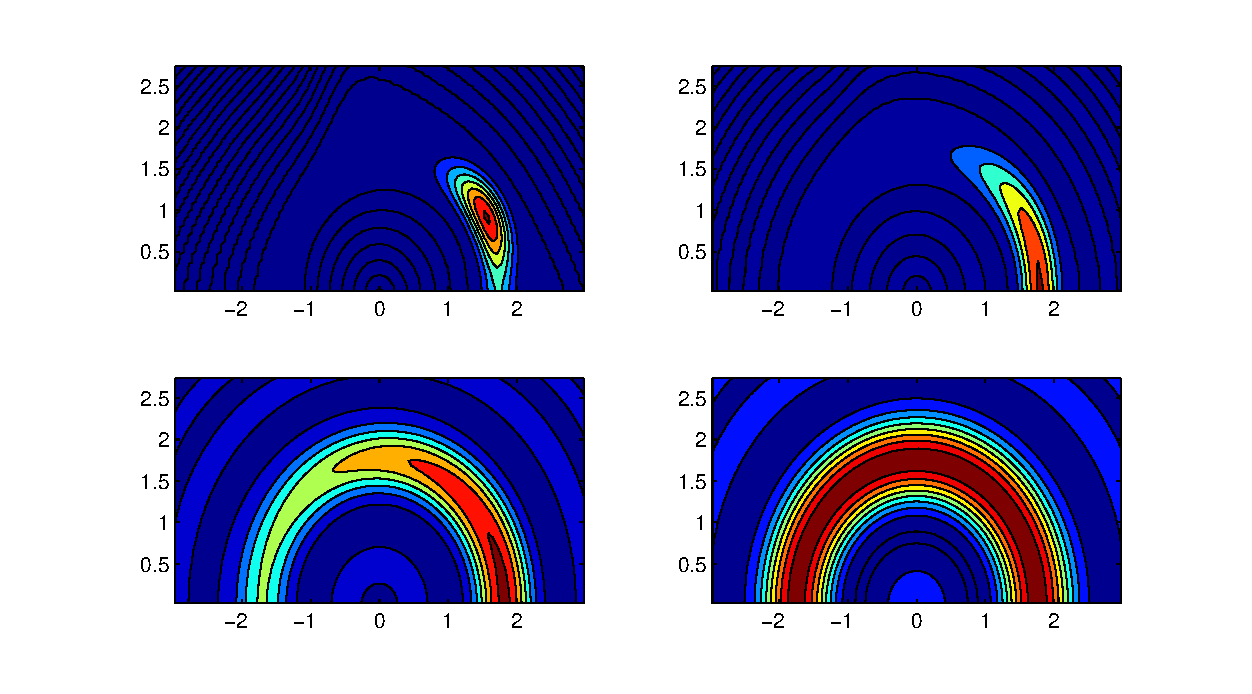
\includegraphics[width=0.9\textwidth]{pitchangle.eps}
\caption{Snapshot of velocity space as three different time intervals showing the effect of pitch angle scattering on the velocity space.  Coordinates are $v_{\parallel}$ horizontally and $v_{\perp}$ vertically. All data shown in this chapter was run with 100 parallel velocity points and 50 $\mu$ points non-equally spaced.\label{pitch-angle}}
\end{center}
\end{figure}

\subsubsection{Energy scattering}

This effect is switched on by setting \texttt{en\_scatter} $=$ \texttt{.true.} in the collisions input deck.  The energy scattering term spreads the distribution function in energy.

\begin{figure}[h!]
\begin{center}
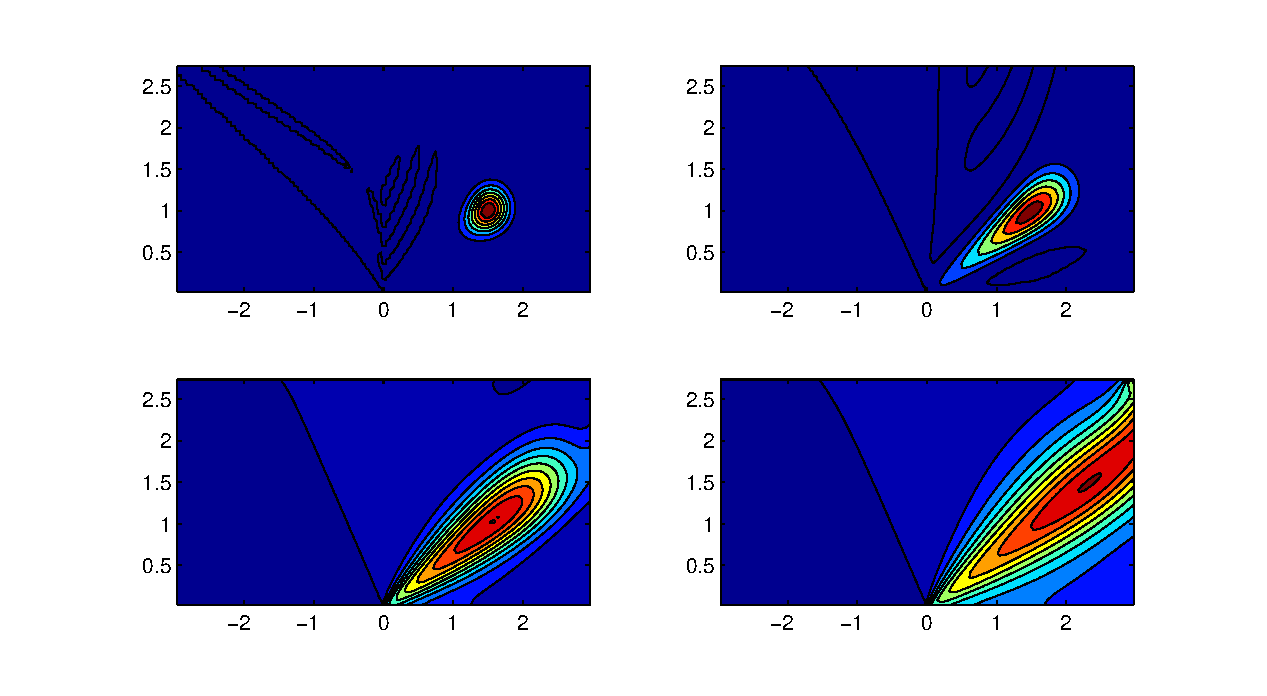
\includegraphics[width=0.9\textwidth]{enscatter.eps}
\caption{Snapshot of velocity space as four different time intervals showing the effect of energy cattering on the velocity space. Coordinates are $v_{\parallel}$ horizontally and $v_{\perp}$ vertically. }
\end{center}
\end{figure}

\subsubsection{Collisional friction}

This effect is switched on by setting \texttt{friction\_coll} $=$ \texttt{.true.} in the collisions input deck.  The collisional friction term advects the distribution function towards the origin in velocity space.


\begin{figure}
\begin{center}
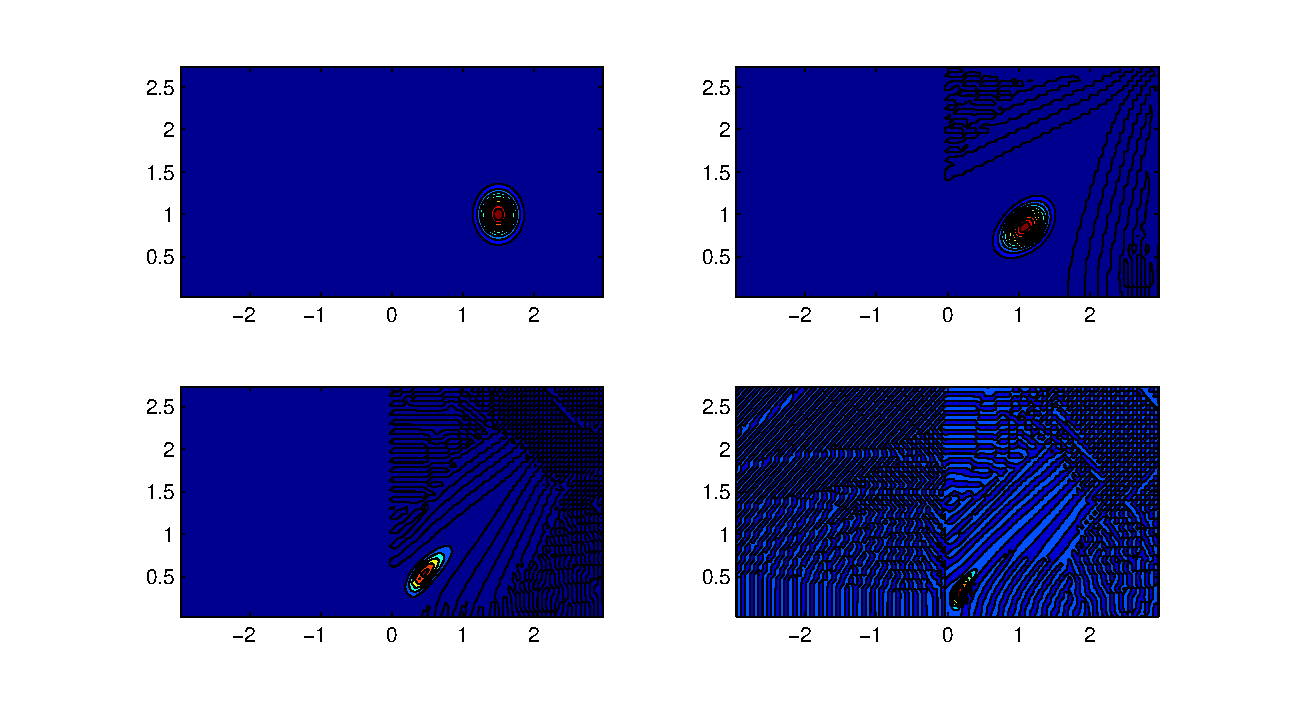
\includegraphics[width=0.9\textwidth]{collfric.eps}
\caption{Snapshot of velocity space at four different time intervals showing the effect of the collisional friction term on the velocity space.}
\end{center}
\end{figure}

When you combine all three effects we get an evolution of the distribution function towards a maxwellian centred on zero and with a width of a single normalized thermal velocity.

\begin{figure}
\begin{center}
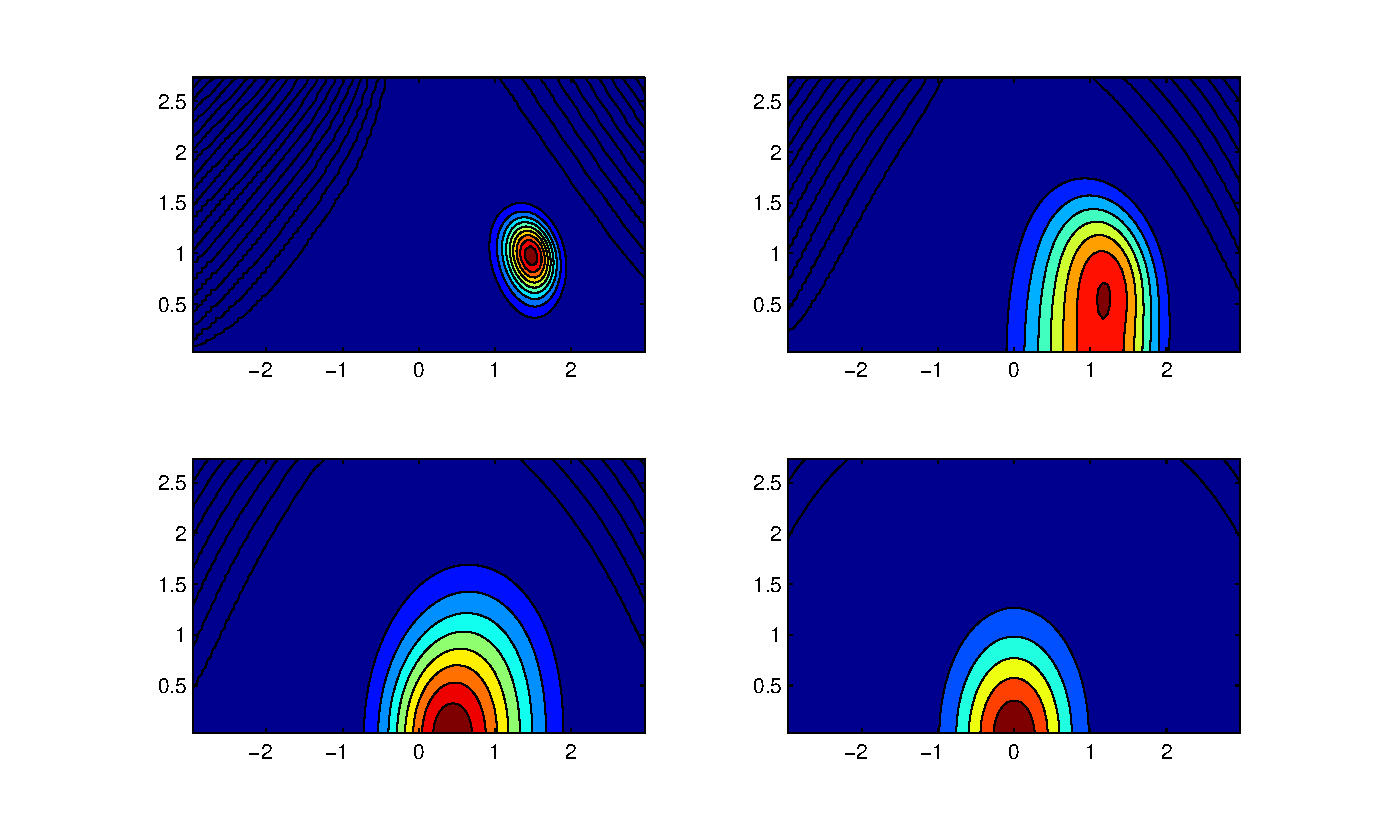
\includegraphics[width=0.9\textwidth]{fulloper.eps}
\caption{Snapshot of velocity space as four different time intervals showing the effect of all the terms in the collison operator on the velocity space.  The final state is a maxwellian centred on zero.}
\end{center}
\end{figure}

\subsection{Velocity space boundary conditions}

There are currently two options for the boundary conditions in velocity space.  The input deck parameter \texttt{mass\_conserve} changes between open boundary conditions (when set to \texttt{.false.} and zero flux boundary conditions when set to \texttt{.true.} the former being slightly more physical, but the latter being desireable also.  Conservation is down to machine precision when the mu grid is uniform which is not the default.  When the mu grid is non-unifom (which is the usual case unless changed at compile time in velocity\_grid) the mass is conserved down to the fifth decimal place, although this can improve if a greater resolution is used.

\subsection{User defined collision-frequencies}

The collision frequency can be defined in two ways.  Firstly by specifying \texttt{nref} which is the particle density in units of $10^{19}$ particles per $m^{3}$, \texttt{tref}, the temperature in keV and \texttt{rref} which is the toroidal major radius.  These parameters are what the corresponding parameters are normalized to in the code and are never usually specified.  The normalized collision (normalized to the ratio of the thermal velocity to the major radius) frequency is given by,

\be 
\Gamma^{a/b}_N = {R_{\rm ref} n_b Z_a^2 Z_b^2 e^4 \ln \Lambda^{a/b} \over 4 \pi \epsilon_0^2 m_a^2 v_{tha}^4} = 
6.5141\cdot 10^{-5} {R_{\rm ref} n_{\rm ref}^{19} \over T_{\rm ref}^k}  {n_{Rb} Z_a^2 Z_b^2 \ln \Lambda^{a/b} 
\over T_{Ra}^2}
\ee

However if \texttt{freq\_override} $=$ \texttt{.true.} then,

\be
\Gamma^{a/b}_N =  n_b Z_a^2 Z_b^2 \nu_{\rm ref} n_b \Lambda^{a/b}/ T_{Na}^2 \Lambda^{i/i}
\ee

Where $\nu_{\rm ref}$ is the user defined frequency defined as \texttt{coll\_freq} in the input deck.  This is assumed to be the single charged ion - ion (proton/deuteron) collision frequency.  To get agreement with the first method this can be set to $6.5141\cdot 10^{-5}R_{\rm ref}n_{\rm ref}\Lambda^{i/i}/T_{\rm ref}^{2}$.  This value is then scaled to all the other species respectively.  For this to work the first species in the input deck should be singly charged ions.

\begin{footnotesize}
\begin{verbatim}
&COLLISIONS
 rref = 1   !reference major radius
 tref = 1   !reference temperature in units of kev
 nref = 1   !reference density in units 10^19 m^-3
 pitch_angle = .true.           !Switches for the pitch angle scattering
 en_scatter = .true.            !Energy scattering term 
 friction_coll = .true.         !Collisional friction term
 mom_conservation = .false.     !Use the correction to conserve momentum
 mass_conserve = .true.,        !Forces zero flux boundary conditions on velocity space
 freq_override=.false.          !Manually specify ii collision frequency to override ref values
 coll_freq=6.515E-5             !Ion-ion collision frequency used if freq_override=.true. 
\end{verbatim}\end{footnotesize}



\section{E x B background shear}%Last updated by Francis Jul 2009

%From CPC paper.\section{Background $E \times B$ shear flow}
The co-moving system employed in GKW corresponds to a frame that rotates as a rigid body with constant frequency 
$\Omega$. 
The possible radial gradient in the toroidal rotation is then treated through a radial gradient in the averaged parallel velocity 
of the background. 
The radial gradient of the perpendicular velocity has so far been ignored, but is known to play an important role in the 
saturation of the turbulence. 
The sheared $E\times B$ velocity leads to a stabilisation of turbulence through the breaking up of eddy structures. 
This $E\times B$ shearing is always present for a purely toroidally rotating plasma but can, of course, also be related 
to a sheared poloidal rotation. 
In this section it is described how the $E \times B$ shearing is treated in GKW.  

The equilibrium $E \times B$ rotation 
\be
{\bf v}_s(\psi)= {{\bf b} \times \nabla \Phi \over B} 
\ee
lies inside the flux surface.  The shearing rate in the normalised units is defined to be 
\be
\gamma_{E}^N = {1 \over 2}\rho_*^2 {\partial^2 \Phi_N \over \partial \psi^2} ,
\label{gamma_E}
\ee
where the normalisation $\Phi= \rho_* {T_{\rm ref} \over e}\Phi_N$ is as for the
perturbed potential Eq.~(\ref{phi_norm}).  The factor $1/2$ is present due to the definition of the
reference thermal velocity.
In physical units the shearing rate is
\begin{equation}
\gamma_E = {v_{\rm thref} \over R_{\rm ref}} \gamma_E^N = 
{1 \over B_{\rm ref}}{\partial^2 \Phi \over \partial r^2} ,
%Contingent on \phi=r/R_{ref}
%True if r = R_{max}-R_{min}
\end{equation}
where $r=(R_{\rm max}-R_{\rm min})/2$.  The GKW shearing rate is assumed
radially constant and is defined as a flux function.  At the radial centre of the flux tube
$\bf{v_s}$ is chosen to be zero, with the result that there is no net flow over the domain.  In the
local limit with the approximations of the `$s-\alpha$' model geometry
the shearing rate is then equivalent to the familiar definition \cite{Hahm95,Burrell97}:
\begin{equation}
\gamma_E \approx {(RB_p)^2 \over B_t}{\partial^2 \Phi \over \partial \Psi^2}
\approx {d v_s \over d r} .
\end{equation}
As before the index $N$ is dropped in what follows.
The sign convention here is opposite to Eq.~(\ref{gradients}), so $\gamma_E<0$ corresponds to 
$\nabla E_0$ radially outwards.

Only the Doppler shift of the background $E \times B$ rotation is kept in the description, i.e. the
background $E\times B$ rotation is 
added as an additional convective term for the perturbed distribution (${\bf v}_s \cdot \nabla g$) in the gyrokinetic equation~(\ref{complete_set_eq}), 
and we neglect the acceleration due to the background potential.  
With zero net flow across the flux tube one obtains
\be
\label{IX}
{\rm IX} = -{\bf v}_s \cdot \nabla g \rightharpoonup - \rho_*^2 {\partial \Phi \over \partial
\psi}{\mathcal E}^{\psi \zeta}{\partial g \over \partial \zeta} =
 - 2 {\gamma_E \psi}{\mathcal E}^{\psi \zeta}  {\partial g \over \partial \zeta} .
\ee
Defining $\bar \gamma_E= 2 \gamma_E {\mathcal E}^{\psi \zeta} $ and taking the Fourier transform, the term can be written as a derivative in
Fourier space
\be 
{\mathcal T}(-{\bar \gamma_E \psi}{\partial g \over \partial \zeta}) = \bar \gamma_E
k_\zeta {\partial \hat g \over \partial k_\psi} .
\ee
The derivative represents a continuous advection (and shearing) in Fourier space in $k_\psi$.  

There are a number of subtleties associated with numerical evaluation of this derivative. A finite difference approximation cannot resolve the fine 
scale structure in Fourier space.  The `harmonic derivative' \cite{Waltz94,Miller94} is a full convolution over all modes and is equivalent to a
pseudo-spectral implementation using FFTs (as was used for the nonlinear term in Eq.~(\ref{nl_term})).  
Although it correctly implements the $E \times B$ shearing term inside the computational domain, it does not represent a homogeneous shear 
flow because the flow profile does not satisfy the periodicity of the discrete Fourier transform; any turbulent structure passing through the radial
boundary will experience a discontinuity in the flow profile (which in the periodic domain has a sawtooth form).  
Since the local limit requires that the turbulence has no preference for the boundary, periodicity at the boundary must be preserved. 
The `shear-periodic' boundary condition \cite{Baron82,Schumann85,Gerz89} that moves with the mean flow accomplishes this for a finite 
difference representation in the radial direction, but does not naturally translate to the spectral representation.

In coordinates that move with the flow  \cite{Rogallo81,Zang88,Pumir96}, the `radial' wavenumbers become time dependent:
\bee
\psi^\prime = \psi , &\qquad& \qquad \zeta^\prime=\zeta-\psi \bar \gamma_E t ,\\
k_\zeta^\prime = k_\zeta , &\qquad& \qquad  k_\psi^\prime = k_\psi - k_\zeta \bar \gamma_E t .
\eee
In these coordinates, the derivative in Fourier space becomes part of the time derivative.

For a gyro-kinetic code, a time dependent wave vector requires the re-evaluation of the linear terms and Bessel functions at every time-step
and would be computationally prohibitive. 
By discretising the time dependence of the wavenumbers as a remapping of the solution vector between the original fixed wavevectors, 
this expensive re-evaluation can be avoided \cite{HammettAPS06}. 
Using only the fixed wavevector grid, the advection in Fourier space occurs in jumps only when the boundary periodicity is satisfied for a 
given mode. 
Explicitly, the remapping $\hat g (k_\psi, k_\zeta,s) \rightarrow \hat g (k_\psi-\Delta k_\psi, k_\zeta,s)$ occurs when
\be
k_\zeta \bar \gamma_E(t-t_{\rm last remap}) = \Delta k_\psi /2 .
\ee
At the high $k_\psi$ limit the solution vector is discarded.  
This means that the method is non conservative, but since the turbulence is characterised by a peaked spectrum 
(Fig.~\ref{cyclone_linear}), the losses are negligible if the range of radial wavenumbers is suitably wide.  
For numerical stability, the remapping must occur at the same time for all points along the flux tube. 
As the metric tensor ${\mathcal E}^{\psi \zeta}$ is a flux function, see Eq.~(\ref{efun_cst}), this condition is always satisfied for a 
constant shear rate along the field line.

The method in GKW differs from the standard spectral methods to model homogeneous shear flows in fluid turbulence of
Refs.~\cite{Rogallo81,Zang88,Pumir96}, where the wavenumbers must be recalculated and re-meshing occurs for all wavevectors 
at the same time. 
In GKW the method used is the one proposed by Hammett et al. in Ref.~\cite{HammettAPS06}.  
Here the `re-meshing' occurs continually (and at different times for each $k_\zeta$), and the wavenumbers stay on their original fixed grid.  
The accuracy of the method has been argued to be second order on average \cite{HammettAPS06} and
is able to capture the physics effects of a 
background shear flow whilst allowing the desirable features of the flux tube model to be retained.
 
Convergence of the remap method can be (and should be) checked (particularly by for the modes with lowest $k_\zeta$) by decreasing 
$\Delta k_\psi / k_{\zeta {\rm min}}$ (increasing $N_x$ whilst holding $N_{\rm mod}$ constant (defined in the next section)).

%As in CPC paper:
% For purely toroidal rotation (with no poloidal flows) the poloidal components of the parallel flow
% $u_\parallel=R\Omega B_t / B$ and the 
% $E \times B$ flow ${\bf v}_s$ must cancel:
% \be
% v_s = - {B_p \over B_t}u_\parallel = - {B_p R\Omega \over B} . 
% %YC = - {B_p u\over B}
% \ee
% For $s_B=1$, $v_s>0$ indicates a flow in increasing poloidal direction, ${\bf v}_s\cdot \nabla
% \theta>0$. 
% For $s_j=1$, ${\bf B}\cdot \nabla \theta>0$, with the poloidal component of the magnetic field
% positive, $B_p>0$. 
% For the gradients
% \be
% \gamma_E = - {\partial \over \partial \psi} \left({B_p R_{\rm ref} \over |\nabla
% \psi|}\Omega\right) \approx  {B_p u^\prime \over B} ,
% \ee
% since the definitions (\ref{gradients}) and (\ref{gamma_E}) have opposite sign.  

%FC: I have sketches as jpeg to illustrate both sign and general geometry coupling.

%FC: Post CPC paper - Oct 09
\subsection{Purely toroidal sheared rotation in general geometry}

Here we follow the notation in Peeters (2009) on centrifugal effects \cite{PEE09}
and the normalisations and definitions of the CPC paper.  We also note that by definition
$\vec{\Omega}=-s_B \Omega \nabla z$.  We denote the plasma rotation with $\omega(\psi)$ and the
rigid frame rotation with $\Omega$, with both normalised by $v_{\rm thref} / {R_{\rm ref}}$.  Note
that in the CPC paper no distinction is made, but here we use both to avoid ambiguity.

In the case of purely toroidal rotation (in the laboratory frame in non-normalised units)

\begin{equation}
u_\parallel \vec{b} + {\bf v}_s  = s_B R \omega(\psi) R \nabla \phi
\label{toroidal}
\end{equation}
where $\phi$ is the toroidal angle.  From the normalisation definitions above one can show that
\begin{equation}
 {\bf v}_s = \left({1 \over 2} \rho_*^2 v_{\rm thref}\right) {\vec{b} \times \nabla_N \psi \over
B_N} {\partial \Phi^N \over \partial \psi}
\end{equation}
hence in the normalised units, taking the bi-normal component of \ref{toroidal} one finds
\begin{equation}
 u_{\parallel N} \underbrace{\vec{b} \cdot \nabla_N \zeta}_{=0} +  {1 \over 2}
\rho_*^2 \underbrace{{\vec{b} \times \nabla_N \psi \over B_N}\cdot \nabla_N
\zeta}_{=\mathcal{E}^{\psi \zeta}}{\partial \Phi_N \over \partial \psi} = s_B R_N^2 \omega_N(\psi)
\underbrace{\nabla_N \phi \cdot \nabla_N \zeta}_{=-1/2\pi R_N^2}
\end{equation}
hence
\begin{equation}
 {1 \over 2} \rho_*^2 {\partial \Phi_N \over \partial \psi} = - {s_B \over 2 \pi}{1 \over
\mathcal{E}^{\psi \zeta}}\omega_N(\psi)
\end{equation}
taking the radial derivative
\begin{equation}
 {1 \over 2} \rho_*^2 {\partial^2 \Phi_N \over \partial \psi^2} = - {s_B \over 2 \pi}\left({1 \over
\mathcal{E}^{\psi \zeta}}{\partial \omega_N \over \partial \psi} + \omega_N{\partial \over \partial
\psi} \left({1 \over \mathcal{E}^{\psi \zeta}}\right)\right)
\end{equation}
Finally we transform to the rotating (starred) frame in which
$\omega_N^*(\psi)=\omega_N(\psi)-\Omega_N$ such that $\omega_N^*(\psi)=0$ (and hence ${\bf
v_s}=0$)
at the centre of the radial domain.  Since the frame rotates rigidly, ${\partial \Omega_N \over
\partial \psi}=0$. The tensor $\mathcal{E}$ is invariant under the transformation (check??).  The
electric field in the rotating frame transforms \cite{PEE09} to 
\begin{equation}
\Phi_N^*=\Phi_N + \underbrace{s_B s_j}_{check ??}{2 \over \rho_*^2}\Psi_N \Omega_N 
\end{equation}
where $\Psi = R_{\rm ref}^2 B_{\rm ref}\Psi_N$ is the poloidal flux and the factor of $2 /
\rho_*^2$ arises from the normalisation of $\Phi$.  In the rotating frame the coupling condition
becomes
\begin{equation}
 \underbrace{{1 \over 2} \rho_*^2 {\partial^2 \Phi_N^* \over \partial \psi^2}
-\underbrace{s_B s_j}_{??}  \underbrace{\Omega_N}_{ \rm VCOR} \overbrace{\partial^2 \Psi_N \over
\partial \psi^2}^{\rm New: d2pffun}}_{\rm
SHEAR\_RATE^{LAB}} = - {s_B \over 2 \pi}{1 \over
\mathcal{E}^{\psi \zeta}}\underbrace{\partial \omega_N^* \over \partial \psi}_{\rm UPRIM} +
\Omega_N{\partial \over \partial \psi} \left({1 \over \mathcal{E}^{\psi \zeta}}\right) 
\end{equation}
Since $\Psi=f(\psi)$ only, from the relation 
\begin{equation} 
{\cal E}^{\psi \zeta} = \frac{s_{\rm j}}{4\pi}\frac{\partial \psi}{\partial \Psi_N}
\label{efun_cst}
\end{equation}
it follows that
\begin{equation}
 {\partial \over \partial \psi} \left({1 \over \mathcal{E}^{\psi \zeta}}\right) = s_j 4 \pi 
{\partial^2 \Psi_N \over \partial \psi^2}
\end{equation}
hence
\begin{equation}
 \underbrace{{1 \over 2} \rho_*^2 {\partial^2 \Phi_N^* \over \partial \psi^2}}_{\rm SHEAR\_RATE^*}
+s_B s_j \underbrace{\Omega_N}_{\rm VCOR} {\partial^2 \Psi_N \over
\partial \psi^2} = - {s_B \over 2 \pi}{1 \over
\mathcal{E}^{\psi \zeta}}\underbrace{\partial \omega_N^* \over \partial \psi}_{\rm UPRIM}
\end{equation}
All quantities in the above equation are flux functions, and the shear rate will always be a
flux function as required for the discrete remapping method.   At version 1135 this
\texttt{TOROIDAL\_SHEAR} coupling is only implemented for \texttt{VCOR}=0.

\begin{footnotesize}
\begin{verbatim}

&ROTATION	       !Namelist read in rotation.F90 -> read_rotation
 VCOR = 0.0            !Rotation of the plasma vcor = Rref Omega / vthref
                       !Always in direction of toroidal magnetic field if positive.
 shear_rate = 0.3      !Normalised shearing rate for the E x B perpendicular shear 
 shear_profile  = 'none'    !To include a shear flow, use `wavevector_remap'
                            !discrete mapping of wavevectors (use NX >> NMOD ) 
 toroidal_shear = 'none'    !Override uprim inputs to be toroidally consistent with shear_rate
                            !'use_uprim': shear_rate derived from input uprim for species 1.
                            !'use_shear_rate': uprim derived from input shear_rate.
/
\end{verbatim}
\end{footnotesize}



\begin{thebibliography}{10}


\bibitem{LIT83} R. G. Littlejohn, J. Plasma Phys. {\bf 29}, 111 (1983).
\bibitem{HAH88} T. S. Hahm, Phys. Fluids {\bf 31}, 2670 (1988)
\bibitem{BRI88} A. Brizard, Phys. Plasmas {\bf 41}, 541 (1988)
\bibitem{SUG00} H. Sugama, Phys. Plasmas {\bf 7}, 466 (2000).

\bibitem{KAR86} C.F.F. Karney, {\sl Fokker-Planck and quasi-linear codes}, Comp. Phys. Reports {\bf 4} 183 
(1986) 
% E x B shear method
\bibitem{Hahm95}
T.~S. Hahm and K.~H. Burrell.
\newblock {\em Phys. Plasmas}, {\bf 2} (1995) 1648

\bibitem{Burrell97}
K.~H. Burrell.
\newblock Phys. Plasmas, {\bf 4} (1997) 1499

\bibitem{Waltz94}
R.~E. Waltz, G.~D. Kerbel, and J.~Milovich, Phys. Plasmas {\bf 1} (1994) 2229

\bibitem{Miller94}
R.~L. Miller and R.~E. Waltz, Phys. Plasmas {\bf 1} (1994) 2835

\bibitem{Baron82}
F.~Baron. {PhD} in physics, (Univ. Pierre et Marie Curie, Paris, France, 1982) 

\bibitem{Schumann85}
U.~{Schumann}, {Algorithms for direct numerical simulation of shear-periodic
  turbulence}, in {\em Lecture Notes in
  Physics {\bf 218}} (Berlin Springer Verlag 1985) pages 492

\bibitem{Gerz89}
T.~Gerz, U.~Schumann, and S.~E. Elghobashi, Journal of Fluid Mechanics Digital Archive {\bf 200} 
(1989) 563

\bibitem{Rogallo81}
R.~S. {Rogallo}, {\em Numerical experiments in homogeneous turbulence}.
\newblock {\em NASA STI/Recon Technical Report N} (1981) 81:31508

\bibitem{Zang88}
T.~A. {Zang}, Applied Numerical Mathematics {\bf 7} (1991) 27

\bibitem{Pumir96} Alain Pumir, Phys. Fluids, {\bf 8} (1996) 3112

\bibitem{HammettAPS06}
G.~W. {Hammett}, W.~{Dorland}, N.~F. {Loureiro}, and T.~{Tatsuno}.
\newblock {Implementation of Large Scale E x B Shear Flow in the GS2
  Gyrokinetic Turbulence Code}.
\newblock {\em APS Meeting Abstracts} (2006) pages 1136 % E x B shear method
\bibitem{Hahm95}
T.~S. Hahm and K.~H. Burrell.
\newblock {\em Phys. Plasmas}, {\bf 2} (1995) 1648

\bibitem{Burrell97}
K.~H. Burrell.
\newblock Phys. Plasmas, {\bf 4} (1997) 1499

\bibitem{Waltz94}
R.~E. Waltz, G.~D. Kerbel, and J.~Milovich, Phys. Plasmas {\bf 1} (1994) 2229

\bibitem{Miller94}
R.~L. Miller and R.~E. Waltz, Phys. Plasmas {\bf 1} (1994) 2835

\bibitem{Baron82}
F.~Baron. {PhD} in physics, (Univ. Pierre et Marie Curie, Paris, France, 1982) 

\bibitem{Schumann85}
U.~{Schumann}, {Algorithms for direct numerical simulation of shear-periodic
  turbulence}, in {\em Lecture Notes in
  Physics {\bf 218}} (Berlin Springer Verlag 1985) pages 492

\bibitem{Gerz89}
T.~Gerz, U.~Schumann, and S.~E. Elghobashi, Journal of Fluid Mechanics Digital Archive {\bf 200} 
(1989) 563

\bibitem{Rogallo81}
R.~S. {Rogallo}, {\em Numerical experiments in homogeneous turbulence}.
\newblock {\em NASA STI/Recon Technical Report N} (1981) 81:31508

\bibitem{Zang88}
T.~A. {Zang}, Applied Numerical Mathematics {\bf 7} (1991) 27

\bibitem{Pumir96} Alain Pumir, Phys. Fluids, {\bf 8} (1996) 3112

\bibitem{HammettAPS06}
G.~W. {Hammett}, W.~{Dorland}, N.~F. {Loureiro}, and T.~{Tatsuno}.
\newblock {Implementation of Large Scale E x B Shear Flow in the GS2
  Gyrokinetic Turbulence Code}.
\newblock {\em APS Meeting Abstracts} (2006) pages 1136 

\bibitem{PEE09} A.G. Peeters, D. Strintzi, C. Angioni, et al., Phys. Plasmas {\bf 16} (2009) 042310


\end{thebibliography}



\chapter{Tearing modes}

Here are some brief notes that describe how a magnetic island is included in the current version of GKW.

If we initially assume a constant poloidal flux perturbation with a given helicity 
\be 
A_\parallel = C \exp [ 2 \pi {\rm i} (m s - n \gamma ) ] 
\ee 
where s and $\gamma$ are the poloidal and toroidal angles, respectively.  If we introduce the helical coordinate $\zeta = qs - \gamma$ and expanding the safety factor up to first order
\be 
q = m / n + \psi\partial q /\partial\psi
\ee 
in the centre of the box (i.e. the mode is resonant at this position). We need to transform this
representation to the ($\psi, \zeta, s)$ coordinate system which gives,
\be 
A_\parallel = C \exp [ 2 \pi {\rm i} ( n \zeta - {\partial q \over \partial \psi} n s \psi ) ] 
\ee 
From which it directly follows that 
\be 
k_\zeta = 2 \pi n \rho_* 
\ee
From the periodicity contraint connected with the parallel boundary conditions it then follows 
that we have to keep radial modes with ($N = ikxspace$),
\be 
k_\psi = (p/N) k_\zeta {\partial q \over \partial \psi} = (p/N) 2 \pi n \rho_* {\partial q \over \partial \psi} 
\ee 
where $p$ is an integer. From $p = 1$ one directly obtains the radial size of the box 
\be 
\psi \rightarrow \biggl [ - { N \over 2 n \partial q / \partial \psi} , {N \over 2 n \partial q / \partial \psi} \biggr ]  
\ee

The Fourier amplitudes of the the different radial modes then can be calculated by integrating over 
the radial domain 
\be 
\hat{A}(k_\psi, k_\zeta, s) = C \int {\rm d} \psi \exp \biggl [ - 2 \pi {\rm i} n {\partial q \over \partial \psi}
\psi [ p + s] \biggr ] 
= {C N \over \pi n \partial q / \partial \psi} {\sin [ \pi (p + Ns) ] \over p + Ns } 
= C^*N {\sin [ \pi s^\circ ] \over s^\circ} 
\ee 
where we have use the ballooning angle $s^\circ = N*s + p$ in the last step.

One point to note at this point is that this perturbation is not periodic in the domain of GKW for all values of s.  This manifests itself as a discontinuity in the parallel vector potential at the edge of the computational domain.  A solution to the this problem is to relax the constant flux approximation and therefore write the perturbation as,
\be 
A_\parallel = C \exp{\imath k_{\zeta}\zeta}\sum_{p=0}^{\inf} A^{p}(s)\exp{\imath pk_{\psi}\psi}
\ee  
Where $A^{p}(s)$ is a damping function.  We have chosen a Gaussian profile to reduce any ringing.  This gives,
\be
\exp{\left((-(sN+p)^{2}/L^{2})\right)}\frac{\sin{\pi(sN+p)}}{\pi(sN+p)}
\ee
Where L is half width of the gaussian envelope (This is set to 2.0 by default).  This approximation of the leads to a more satisfactory shape for the vector potential, where the value of L can be tuned to that the damping of the small k modes is negligible and the of high k modes sufficuiently strongly to prevent the occurance of a jump at the boundary.

Thus the full vector potential has the form,

\be
A_{||} = C\exp{(\imath k_{\zeta}\zeta - \imath\omega t)}\sum_{p=-Nx/2}^{p=Nx/2}\exp{\left(-\frac{(sN+p)^2}{L^2}\right)}\frac{\sin{(\pi(sN+p))}}{\pi(sN+p)}\exp{(\imath p k_{\psi}\psi)}
\ee

Note that only a single binormal mode is used.  The island width, W, is converted to the vector potential by using the expression,
\be
w = 2\sqrt{\left[\frac{rqB_{r}}{mB_{\theta}(dq/d\psi)}\right]}
\ee
where $B_{\phi}$ and $B_{\theta}$ is the toroidal and poloidal components of the magnetic field respectively.  $dq/d\psi$ is the magnetic shear and n is the poloidal mode number.  Furthermore we use the fact that the radial magnetic field is prescribed as $B_{r}= m\tilde{\psi} /rR$, and that in a circular cross-section plasma equilibrium the perturbed magnetic flux is given by $\tilde{\psi} = R\tilde{A_{\parallel 0}}$.  This allows us to prescribe the correct island width within GKW which is normalised by $\rho_{ref}$ to give the parameter wstar.

\begin{figure}
\begin{center}
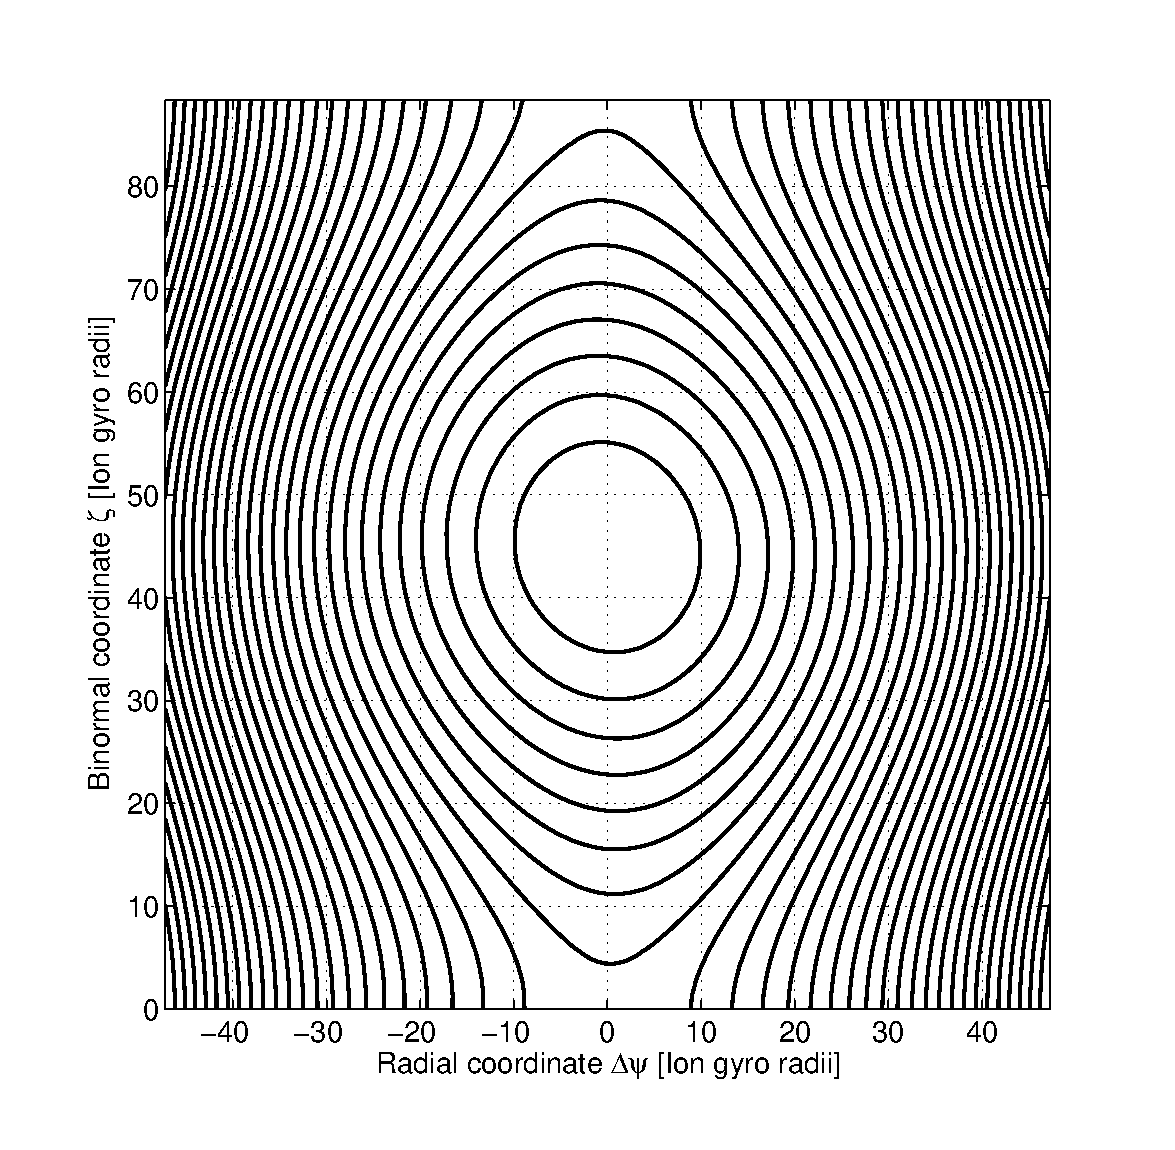
\includegraphics[width=0.45\textwidth]{MagIslGeom.eps}
\caption{Magnetic Island Geometry for an island with a half width of 30 ion gyro-radii}
\label{islandgeom}
\end{center}
\end{figure}

To run GKW with a magnetic island present the following options must be used.  Firstly the code must be set to run electro-magnetically by setting {\bf nlapar}$=$.true..

In the spcgeneral common block, {\bf finit} must be set to {\it island}, which adds the magnetic island as a perturbation of the equilibrium field.  A further input parameter is the rotation frequency of the island, which is set by the parameter {\it isl\_rot\_freq} which must be entered normalised, when plotting XY profile outputs, setting {\it list\_follow} in the diagnostic namelist will follow the magnetic island so that the O-point is always in the centre of the box.

\begin{verbatim}
 &SPCGENERAL
 beta = 0.0001,
 finit = 'island',
 wstar = 5.0
 adiabatic_electrons = .false.
 Ls = 2.0,
 isl_rot_freq = 0.1,
 /
\end{verbatim}

The half width of the island is determined by the input parameter {\bf wstar} which is the island width normalised to the ion gyro-radius.  A point of note is that this island width can not exceed the radial extent of the computational box due to the periodicity constraints of being a pseudo-spectral code.

\subsection{Profile flattening in GKW}

The full benchmark of the magnetic islands implementation requires the flattening of the temperature and density profiles.  The equilbrium profiles are linear and are present in the source terms.  Since we are solving for the perturbed part of the distribution function, the solution should respond to the source terms due to the background gradients and the magnetic island giving a perturbuation that cancels the background out through the islands O-point.

Runs must be non-linear for the correct level of flattening to be obtained.

\subsubsection{Reconstruction of radial density and temperature profiles}

To reconstruct the radial density profile firstly the XY diagnostics must enabled in the diagnostics namelist.

\begin{verbatim}
&DIAGNOSTIC
 lisl_follow = .false.,
 lphi_diagnostics = .true.,
 xy_phi = .true.,
 xy_apar = .true.,
 xy_fluxes = .true.,
 xy_fluxes_em = .true.,
 xy_dens = .true.
 xy_current = .true.,
 xy_temp = .true.,
 / 
\end{verbatim}

The files named Densi000*\_* hold the XY perturbed density data ($\tilde{n}$) for each large time step.  The background density profile can be reconstructed by using the date in the filed named {\it xphi} (Radial coordinate values same dimensions as XY slices) and the input parameter RLn (different for each species), thus the full density is:
\be
n({\Delta\psi}) = \tilde{n} - RLn*xphi
\ee

The temperature profiles are slightly more complicated.  The files Tempe000*\_* hold the second moments of the distribution function (Energy, $\tilde{E}$), thus to get the perturbed temperature $\tilde{T}$ 
\be
\tilde{T} = (1/n_{ref})(\frac{2}{3}\tilde{E} - T_{ref}\tilde{n})
\ee
which in the same way as the total density, can be made into the total temperature by,
\be
T({\Delta\psi}) = \tilde{T} - RLT*xphi
\ee

\begin{figure}
\begin{center}
\includegraphics[width=0.95\textwidth]{tempflat.eps}
\caption{Radial temperature profiles through the O-point (Blue) and X-point (Red) in the presence of a magnetic island.  With the background (Green) temperature.}
\end{center}
\end{figure}

\cleardoublepage 

%\pagenumbering{arabic}

\vfill \eject 
\hbox to 2 truecm{\hfill}
\vskip 8 truecm 

\centerline{\selectfont \Huge I AM A FREAK} 
\addcontentsline{toc}{chapter}{I AM A FREAK}

\vfill  \eject 


\chapter{Diagnostics} 

\section{fluxes} %This section has been consolidated with the separate one on the fluxes routine
\label{fluxes}
\index{fluxes}

The fluxes are calculated as guiding center fluxes and are given by the equations 
\be 
\Gamma_i^\psi  = \biggl \langle \int {\rm d}^3 {\bf v} \tilde {\bf v}_E\cdot \nabla \psi  \alpha_i f \biggr \rangle 
\ee
where i = (1,2,3) with $\alpha = (1, mv^2/2,v_\parallel)$, i.e. $\alpha = 1$ is the 
particle flux, $\alpha = 2$ is the heat flux and $\alpha = 3$ is the parallel momentum 
flux. The big angle brackets denote the flux surface average. 

Both the potential as well as the distribution function are represented as a sum over 
Fourier modes. Since the flux contains an average over space it will be zero unless 
the wave vectors of the potential and distribution function add up to be zero. In the 
representation of modes used in this manuscript this means that a particular wave 
vector of the representation of $f$ must be combined with the complex conjugate of 
the same wave vector in the representation of $\phi$, i.e.  
\be 
\langle \tilde v_E f \rangle  = 2 \sum_m {\rm Re}  [ \langle \tilde {\bf v}_{Em}^\dagger 
\cdot \nabla \psi  f_n \rangle ]  
\ee 
where $v_{En}$ ($f_n$) is the Fourier amplitude of the ExB velocity (distribution function) 
of the mode $n$, and the dagger denotes the complex conjugate. Substituting the 
various definitions one can derive that a normalized flux can be defined as 
\be 
{\cal I}_i = \sum_m \biggl \{ 2 \pi B {\cal E}^{\psi \beta} k_{\beta m } \int {\rm d} 
\mu {\rm d} v_{\parallel} \,  \alpha_i {\rm Im} [ \langle \phi_m \rangle^\dagger f_m ] \biggr \}
\ee
where $\alpha_i = (1, v_\parallel^2 + 2 \mu B,v_\parallel)$  
This definition means that the fluxes in physical units can be obtained from 
\be 
R_{\rm ref} \Gamma^\psi_s  = n_s \rho_*^2 v_{\rm thref} {\cal I}_1 
\ee 
\be 
R_{\rm ref} Q_s^\psi = n_s T_s \rho_*^2 v_{\rm thref} {\cal I}_2 
\ee 
\be 
R_{\rm ref} \Gamma^\psi_{\phi s} = m_s n_s v_{ths} \rho_*^2 v_{\rm thref} {\cal I}_3   
\ee

\subsection{Details of the routine}
The radial component of the ${\bf E} \times {\bf B}$ velocity and the distribution function are given by 
\be 
\tilde {v}_{Ex} = \sum_k  {\rm i} {k_y \phi_k \over B} {\bf e}_x \exp [ {\rm i} {\bf k} 
\cdot {\bf x} ] + c.c  
\ee
\be 
f = \sum_k f_k\exp [ {\rm i} {\bf k} \cdot {\bf x} ] + c.c  
\ee
Multiplying these two expressions and averaging over space yields 
\be 
v_{Ex} f = 2 \sum_k {k_y \over B} {\rm Im} ( \phi_k^\dagger f_k) 
\ee 
where the dagger denotes the complex conjugate.  

Using all the normalizations that are described in section \ref{normalization} one can 
write the equation in the form 
\be 
\Gamma_i = n_0 \rho_*^2 v_{\rm th} \sum_k \biggl \langle \int {\rm d}^3 v_N^3 \, \alpha_i k_{yN} 
{\rm Im}(\phi^\dagger_{kN}  f_{kN} ) \biggr \rangle  =  n_0 \rho_*^2 v_{\rm th} {\cal I}(\alpha_i)
\ee 
The fluxes in the routine are calculated for every mode and stored in {\texttt pflux, eflux}
and {\texttt vflux}. These are defined as 
\be 
{\texttt pflux} = {\cal I}(1)
\ee
\be 
{\texttt eflux} = {\cal I}(v_N^2)
\ee
\be 
{\texttt vflux} = {\cal I}(v_{\parallel N} ) 
\ee
Consequently in physical units the fluxes are 
\be 
\Gamma = n_0 \rho_*^2 v_{\rm th} {\texttt pflux} 
\ee
\be 
Q = n_0 T_0 \rho_*^2 v_{\rm th} {\texttt eflux} 
\ee
\be 
\Gamma_\phi = m n_0 \rho_*^2 v_{\rm th} {\texttt vflux} 
\ee    
So to get the real flux one still needs to multiply with the density and / or temperature of the particular species.  The normalization, however, has the advantage that the diffusivity coeffcients are
\be
D       = \rho_*^2 L_N v_{\rm thref} pflux
\ee
\be
\chi     = \rho_*^2 L_T v_{\rm thref} eflux 
\ee
\be
\chi_{\phi} = \rho_*^2 L_u v_{\rm thref} v_R vflux
\ee
Note that the momentum flux must be multiplied with the relative velocity. The fluxes contain both the anomalous as well as the neo-classical fluxes. The anomalous flux contains the contributions due to the ExB velocity and the magnetic flutter.

For example from the heat flux output we can calculate the normalized species heat diffusivity
\be
\chi_s^N = {{\texttt eflux} \over R/L_{T_s} } = {R \chi_s  \over \rho_{\rm ref}^2 v_{\rm thref}} 
\ee

For a linear run, the dominant mode growth rate is calculated as
\be
\gamma_{N}^{max}(t_N)={\ln \left[{\sum_m |\hat \phi|^2(t_N) \over \sum_m |\hat \phi|^2(t_N-\Delta t_N)}\right] \over \Delta t_N}
\ee
The mode frequency is calculated as
\be
\omega_N(t_N)=\frac{1}{\Delta t_N}\left(\frac{\sum_s |\hat \phi(t_N)| {\mathrm Arg}({\hat \phi}(t_N))}{\sum_s|\hat \phi(t_N)|} - \frac{\sum_s |\hat \phi(t_N-\Delta t_N)|{\mathrm Arg}({\hat
\phi}(t_N-\Delta t_N))}{\sum_s |\hat \phi(t_N-\Delta t_N)|}\right).
\ee
Positive values indicate propagation in the direction opposite to $\nabla \zeta$ (which for $s_j=1$ is in the ion diamagnetic drift direction).

\begin{table}[h!]
\begin{tabular}{l|l|l|l}
 Filename & Description & Quantity & Cols,(Rows)\\
\hline
time.dat & Dominant linear mode growth rate & $t_N, \gamma_{N}^{max}, \omega_N$ & 3  \\

fluxes.dat & Total fluxes $(i=1,2,3)$ for each species  & ${\cal I}_i=\sum_{k_\zeta} \sum_{k_\psi} \sum_{s} {\cal J}_i$  & $3N_{sp}$ \\

kyspec & Binormal mode potential spectrum &  $\sum_{k_\psi} \sum_{s} |\hat \phi(k_\psi,k_\zeta,s)|^2$    &  $N_{mod}$\\

kxspec & Radial mode potential spectrum &  $\sum_{k_\zeta} \sum_{s} |\hat \phi(k_\psi,k_\zeta,s)|^2$  & $N_x$  \\

{p/e/v}\_flux\_spectra & Binormal spectral flux for each species & $\sum_{k_\psi} \sum_{s} {\cal J}_i(k_\psi,k_\zeta,s) $ & $N_{mod}N_{sp}$ \\

{p/e/v}\_flux\_xspec  & Radial spectral fluxes for each species & $\sum_{k_\zeta} \sum_{s} {\cal J}_i(k_\psi,k_\zeta,s) $  & $N_{mod}N_{sp}$   \\

parallel\_phi.dat & Parallel  potential  & $ \sum_{k_\zeta} \sum_{k_\psi} |\hat \phi(k_\psi,k_\zeta,s)|^2$ & $N_s$        \\

spc\#     & 2D potential spectrum slice \# by timestep & $|\hat \phi(k_\psi,k_\zeta,s=0)|$ & $N_x, (N_{mod})$ \\

phi\#     & 2D potential slice \# by timestep &  $\phi(\psi,\zeta,s=0)$ & $M_x, (M_{mod})$\\

\hline
\end{tabular}
\caption{Time trace diagnostics output by GKW. The coordinate labels for the \texttt{par\#} output are in \texttt{xphi} and \texttt{yphi}.}
\end{table}

\begin{table}[h!]
\begin{tabular}{l|l|l|l}
 Filename & Description & Quantities & Cols,Rows \\
\hline
krho & Binormal wavevector grid & $(q / 2 \pi \psi) k_\zeta \rho_{\rm ref} = k_\perp(k_\psi=0,s=0) \rho_{\rm ref}$ & $N_x, N_{mod}$\\
kxrh & Radial wavevector grid & $k_\psi \rho_{\rm ref}$ & $N_x, N_{mod}$\\
yphi & Real space binormal grid & $ 2 \pi \psi (\zeta-\zeta_{min})/q\rho_{\rm ref}$ & $M_x, M_{mod}$ \\
xphi & Real space radial grid & $(\psi-\psi_{min})/\rho_{\rm ref} $ & $M_x, M_{mod}$ \\
parfun.dat & Perpendicular wavevector & $k_\perp\rho_{\rm ref}, $ & $2,N_s N_{mod} N_x$\\
par.dat & Curvature and Coriolis functions & $k_\perp\rho_{\rm ref}$ , ${\cal D}^\psi k_\psi + {\cal D}^\zeta k_\zeta$ , ${\cal H}^\psi k_\psi + {\cal H}^\zeta k_\zeta$, & $3,N_s N_{mod} N_x$\\
geom.dat & Geometry tensors & Labelled in file & N/A\\
kx\_connect & Parallel boundary connections & Labelled in file & N/A\\
\end{tabular}
\caption{Initial grid diagnostics output by GKW. The grid outputs are scaled so that $\psi$ and $\zeta$ coordinate scales can be compared directly on the input scale of $k_\perp \rho_{\rm ref}$ (see equation \ref{kperp}).} %where $D={\cal D}^\psi k_\psi + {\cal D}^\zeta k_\zeta$, and $H={\cal H}^\psi k_\psi + {\cal H}^\zeta k_\zeta$.
\end{table}

% \begin{table}[h!]
% \begin{tabular}{l|l|l|l}
%  Filename & Description & Quantities & number of columns \\
% \hline
% %distr1.dat &  $v_\parallel$ grid at maximum in potential & $v_\parallel$ & $N_{v\parallel}, &N_{\mu}$\\
% %distr2.dat & $\mu$ grid at maximum in potential & $\mu$ & $N_{v\parallel}, N_{\mu}$ \\
% %distr3.dat & Distribution function for & Im(f(1,1,max,vp,mu)) & $N_{v\parallel}, N_{\mu}$\\
% %distr4.dat & Distribution function for & Re(f(1,1,max,vp,mu)) & $N_{v\parallel}, N_{\mu}$\\
% %parallel.dat & & & \\
% \end{tabular}
% \caption{Final diagnostics ouput by GKW.}
% \end{table}

 \begin{figure}
 \label{directions}
 \begin{center}
 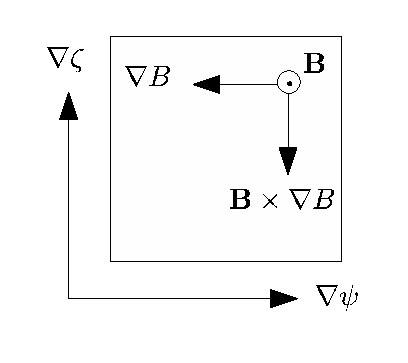
\includegraphics[width=0.5\textwidth]{directions.eps}
 \caption{Coordinate directions on the outboard plane ($s=0$) for $s_B=1$, as output by the potential slices diagnostic \texttt{phi\#} with the coordinate labels for each point as output by \texttt{xphi} and \texttt{yphi} (the yphi coordinate label inverts the plot). For $s_B=1$, the poloidal field is `upwards' ${\rm sign}(B_p \nabla \theta \cdot \nabla \zeta)= s_B$. If in doubt, see Sec.~\ref{signs}.  Note that the `centre' of the flux tube is in the bottom left corner when output from the FFTs.}.

 \end{center}
 \end{figure}
%This means as the matlab script mkmovie plots it. 

\section{Output Files}%Added by FC Apr 2008 - Unfinished - Please improve
\index{output files}
GKW will generate a number of output files depending on the input options and `diagnostic' namelist.  If \texttt{mode\_box = false} the output of potentials is suppressed.

% \begin{footnotesize}
%  \begin{verbatim}
%  &DIAGNOSTIC
%   Add details here.
%  /
% \end{verbatim}
% \end{footnotesize}

\vspace{10pt}
\noindent
The following files are added to or created each data dump timestep (every NAVERAGE timesteps):
\begin{itemize}
\item For a linear run, \texttt{time.dat} contains three columns.  The first is the normalized time, the second is the dominant mode growth rate, and the third is the dominant mode frequency.  If \texttt{CONTROL: normalized=.false.} the third column instead gives the total norm of the distribution function.

\item The columns of \texttt{fluxes.dat} contains the particle flux, energy flux, and momentum flux, (in this order), repeated for each kinetic species in the order of the species input in \texttt{input.dat}.  The file therefore has 3 *(number of kinetic species) columns.

\item The columns of \texttt{\{p/e/v\}flux\_spectra.dat} contain the fluxes toroidal mode (ky) spectra for particle flux, energy flux, and momentum flux \{respectively\}, repeated for each kinetic species.  Therefore each file has NMOD*(number of kinetic species) columns: in for each species for each kinetic species in the order of the species input in \texttt{input.dat}.

\item The columns of \texttt{\{p/e/v\}flux\_xspec.dat} contain the fluxes radial mode (kx) spectra for particle flux, energy flux, and momentum flux \{respectively\}, repeated for each kinetic species.  Therefore each file has NX*(number of kinetic species) columns: in for each species for each kinetic species in the order of the species input in \texttt{input.dat}.

\item \texttt{kyspec} contains the peturbed potential `poloidal' mode spectrum against time.  Plot a slice across the columns for the spectrum at a given timestep.

\item \texttt{spcXXXXXX} Contains the 2D potential spectrum at the outboard side for each dump timestep.

\item \texttt{phiXXXXXX} Contains a 2D real cross section of the potential on the outboard side (can be altered) for each dump timestep.
\end {itemize}

\vspace{10pt}
\noindent
The following files are written at the start of a run:
\begin{itemize}
\item \texttt{input.out} echos the input variables the code is using (including defaults not supplied in the input file). By renaming it to \texttt{input.dat} it could be used for starting the code as if it were \texttt{input.dat}.

 \item \texttt{xphi} and \texttt{yphi} contain real space position information for the data points in the phiXXXXX files.

\item \texttt{krho} contains the values of $k_y\rho$ for each mode. %normalized against $k_{\rm th}^N = q  / ( 2 \pi \psi)$, the normfactor for calculating the $k_\zeta$ values in the code.

\item \texttt{kxrh} contains contains the values of $k_x\rho$ for each mode. %normalized against $k_{\rm th}^N = q  / ( 2 \pi \psi)$, the normfactor for calculating the $k_\zeta$ values in the code.
\end{itemize}

\vspace{10pt}
\noindent
The following files are written once at the end of a successful run:

\begin{itemize}

\item \texttt{parallel.dat} contains some diagnostics connected with the parallel mode structure. For every mode the following quantities are (sequentially) written to file, in this column order:
\begin{verbatim}
sgr         the length along the field line 
phi         the potential 
apar        the parallel component of the vector potential 
dens        the perturbed density 
tpar        the perturbed parallel temperature 
tperp       the perturbed perpendicular temperature 
wflow       the perturbed parallel flow velocity
\end{verbatim}
Note only \texttt{sgr} is real. The other quantities are complex and fill 2 columns in the output file. The file will have $2*N_{MOD}*N_X*N_S$ rows. 

\item \texttt{parfun.dat} and \texttt{par.dat}? contain the curvature and $k_\perp$ function.

\item \texttt{FDSXXXXXX} Contain the distrbution function binaries for each processor needed for restarting a run. The newer restart version will output only 1 binary, \texttt{FDS}.
\end{itemize}


\chapter{Notes on individual routines} 

This chapter discusses the individual routines and gives some details on the physics 
processes implemented. Here, not all the input and output or all the variables are 
discussed. It merely gives some details that should allow the reader to understand
the code better. 

\section{\texttt{linear\_terms.F90}}%Added by Francis Jan 2008
In the treatment so far, the terms as implemented in the code were described in \ref{terms} as terms I-IX. Here we link these terms to the routines in the code, as well as to \ref{g-vlasov}, the Vlasov equation for the modified perturbation distribution function $g$.
\be 
\label{1}
{\partial g \over \partial t} + (\underbrace{v_\parallel {\bf b}}_{I} + \underbrace{{\bf v}_D}_{II} + \underbrace{{\bf v}_\chi}_{III}) \cdot \nabla g  
-\underbrace{{\mu B \over m}{{\bf B}\cdot \nabla B \over B^2}{\partial g \over \partial v_\parallel}}_{IV} = S. 
\ee

Where the source from the Maxwellian background is given by eqn \ref{sources}
\bee 
\label{2}
S &=&  - \underbrace{({\bf v}_\chi}_{V} + \underbrace{{\bf v}_D)}_{VI} \cdot \nabla_p F_M
-  {Ze \over T} \underbrace{[ v_\parallel {\bf b}}_{VII} + \underbrace{{\bf v}_D ]}_{VIII} \cdot \nabla \chi F_M \cr 
\noalign{\vskip 0.2 truecm} 
& & - \underbrace{{Z e \over T} {\mu B \over m} \biggl ( {{\bf B} \cdot \nabla {\bf B} \over B^2} 
\biggr ) \langle A_\parallel \rangle F_M }_{IX}
\eee

We also need the expansion of the drift velocity \ref{drift}
\bee
\label{3}
{\bf v}_D &=& \underbrace{{1\over Ze} \biggl [ \underbrace{{m v_\parallel^2\over B}}_{1} + \underbrace{\mu}_{2} \biggr ] {{\bf B} \times \nabla B
\over B^2}}_{A} + \underbrace{{m v_\parallel^2 \over 2 Z e B} \beta^\prime {\bf b} \times \nabla \psi}_{3} 
 + \underbrace{{ 2 m v_\parallel \over Z e B } {\bf \Omega}_\perp}_{4} \cr 
\noalign{\vskip 0.2 truecm} 
&-& \underbrace{{m \Omega^2 R \over Z e B }  {\bf b} \times {\nabla R}}_{5}, 
\eee

In \texttt {linear\_terms.f90} the various terms from these equations are input into the matrix in individual routines which will be described below.  Most of the computation in the code is done in the wave vector domain. All derivatives in the perpendicular direction are in Fourier space; but derivatives along the field line are done in real space (terms I and VII)

\par
Many of the routines in \texttt {linear\_terms.f90} have two versions (identified by a postfix to the routine name), one for each of the second order and fourth order methods.  We concentrate here on the fourth order method since the other is out of order. The routines do the same thing with regards to which terms are implemented; the implementation is different for each method.  Note that the new distribution $g$ is often called $f$ in the code comments, and its array is called \texttt{fdisi}. Also the normalizations outlined in \ref{normalization} are also used.

\par
\texttt{calc\_linear\_terms} is the master routine that calls the subroutines which put the terms I-IX (excluding term III) into the matrix.  Broadly, the first section puts the terms on the LHS of \ref{1}.  The second section calculates the source terms due to the maxwell background.\ref{2}.  The third section of \texttt{calc\_linear\_terms} calls the routines that input the field equations into the matrix. These are the equations that force the solution the be self consistent with the potentials calculated from the distribution function.  After each section is completed there is a call to \texttt {finish\_matrix\_section} in module \texttt {matdat} which stores the k index labels of the matrix for each section..

\par
Hence \texttt{calc\_linear\_terms} covers all the terms I-IX in \ref{terms} ( also labelled as the underbraced numbers in \ref{1}, \ref{2}, and \ref{3}), with the exception of term III, which is implemented in {\texttt non\_linear\_terms.f90}.

\subsection{\texttt{vpar\_grad\_df}, term I}
\texttt{vpar\_grad\_df} calculates the convection parallel to the field.  This routine also adds parallel velocity dissapation required for a numerically stable solution determined by the dissapation parameter \texttt{disp\_par}.  This term is the free streaming motion along the feild line, with derivative calculated in real space.

\subsection{\texttt{vdgradf}, term II}
\texttt{vdgradf} calculates the drift in the gradient of the eikonal term.

\subsection{\texttt{trapdf}, terms IV and IX}
\texttt{trapdf} calcuates the mirror trapping terms dependent on the switch variable \texttt{trapping}.   This routine also adds perpendicular velocity dissapation required for a a numerically stable solution determined by the dissapation parameter \texttt{disp\_vp}.

\subsection{\texttt{ve\_grad\_fm}, term V}
\texttt{ve\_grad\_fm} calculates the ${\bf E} \times {\bf B}$ drift due to the background distribution, as well as (optionally according to logical \texttt{nlapar}) the electromagnetic correction ${\bf v}_{\delta B_\perp}.$

\subsection{\texttt{neoclassical}, term VI}
\texttt{neoclassical} optionally includes the neoclassical terms according to the switch \texttt{neoclassics}.  Note many gyrokinetics codes disregard this term.

\subsection{\texttt{vpgrphi}, term VII}
\texttt{vpgrphi} calculates the landau damping term, dependent on the switch variable \texttt{landau}.  This is an acceleration along the field line with parallel derivative in real space.

\subsection{\texttt{vd\_grad\_phi\_fm}, term VIII}
\texttt{vd\_grad\_phi\_fm} calculates the  drift in the gradient of phi times the velocity derivative of the Maxwell background.  Note that Equation terms  \ref{3}.1 and \ref{3}.2 are combined as \ref{3}.A in the $E_D$.multiplier as defined in \ref{terms}.

\section{\texttt{non\_linear\_terms.F90}}%Added by Francis Feb 2008

The Fourier amplitudes of the potential (and perturbed distribution function) are defined as 
\be 
\phi_N(x) = \sum_k \phi_{Nk} \exp [ {\rm i} k x ] + c.c.  
\ee 
Note that because the inverse discrete Fourier transform ($H_l$) is defined such that 
the values in real space ($h_n$) are given by  
\be 
h_n = {1\over N} \sum_{l=0}^{N-1} H_l \exp [ {\rm i} 2\pi l n / N ] 
\ee 
where $N$ is the total number of grid points of the discrete transform. The relation between the 
amplitudes and the discrete Fourier transform, therefore, is 
\be 
H_l = N\phi_{Nk}
\ee 
The wave vector $k$ is given by the standard relation  
\be 
k = {2 \pi l \over N \Delta} 
\ee 
where $\Delta$ is the grid distance. This relation is used to determine the size of the box 
in real space. It follows that the lowest non-zero wave vector $k_1$ determines $\Delta$ and
the size of the box $L = N\Delta$ 
\be 
L = {2\pi \over k_1} 
\ee 

\subsection{\texttt{add\_non\_linear\_terms}, term III} 
\index{Non linear terms}
This routine implements the full term III with electromagnetic corrections as described by \ref{electromag}.  Hence the routine finds the ${\bf E} \times {\bf B}$ drift of the perturbed distribution function, and adds the term:
\be 
\label{Edrift}
{\bf v}_E \cdot \nabla g = {{\bf b} \times \nabla \langle \phi \rangle \over B} \cdot \nabla g
\ee
Without the elctromagnetic corrections, Term III of \ref{terms} becomes
\be
\label{nl_term}
{\rm III} = - {\bf v}_\phi \cdot \nabla g \rightarrow - \rho_*^2 {\partial {\langle \phi_N \rangle} \over \partial x_\beta}
{\cal E}^{\beta \alpha} {\partial g_N \over \partial x_\alpha} = {\rho_*^2 {\cal E}^{\psi \zeta}}\left({{\partial {\langle \phi_{N} \rangle} \over \partial \zeta} {\partial g_N \over \partial \psi} - {\partial g_N \over \partial \zeta}{\partial {\langle \phi_{N} \rangle} \over \partial \psi}}\right)
\ee
where the expansion of the tensor sum uses the anti-symmetry of ${\cal E}^{\beta \alpha}$.  Note also that the diagonal elements of ${\cal E}^{\beta \alpha}$ are zero, and derivatives along $s$ are neglected. 

The gyroaveraged potential $\langle \phi_N \rangle$ is first calculated in the wavevector domain by multiplying the potential by the Bessel function $J_0$ (\ref {Bessel}). In k space the derivative of the potential is obtained by multiplying by $ik_\alpha$. 

Hence the implementation in the code is
\be
a = i J_{0}(k_{\perp}\rho) k_{N,\zeta} \phi_{N,k} = ik_{\zeta}\rho_{\rm ref}{\langle \phi_{N,k} \rangle} 
\ee
\be
b = i J_{0}(k_{\perp}\rho) k_{N,\psi} \phi_{N,k} = ik_{\psi}\rho_{\rm ref}{\langle \phi_{N,k} \rangle} 
\ee
Note the $\rho$ in the Bessel function is species dependent.  Also the normalization of the k vector \ref{knorm} $k = {k_N / \rho_{\rm ref}}$ introduces a multiplier of $\rho_{\rm ref}$
Hence the inverse Fourier transformation gives
\be
ar = \mathcal{F}^{-1}(a) =  \rho_{\rm ref} {\partial {\langle \phi_N \rangle} \over \partial \zeta_{N}} = {\rho_{\rm ref} \over R_{\rm ref}} {\partial {\langle \phi_N \rangle} \over \partial \zeta} =  \rho_* {\partial {\langle \phi_N \rangle} \over \partial \zeta}
\ee
\be
br = \mathcal{F}^{-1}(b) =  \rho_* {\partial {\langle \phi_N \rangle} \over \partial \psi}
\ee
%Incorrect, not all corrdinates are normalized the same.
Since the coordinates are normalized by $x_{\alpha,N} = {x_{\alpha} \slash R_{\rm ref}}$.  Here we have explicitly linked the normalizations of the k vector and coordinates to show that under the Fourier transform; $\rho_* {\partial \over \partial x_\alpha} \rightarrow {\rm i} k_\alpha$, as was intended in its definition (see \ref{rho_norm}). Put simply, a factor of $\rho_{*}$ appears after the inverse Fourier transform.

Similarly, the gradient of the distribution function in k space is found $a = i k_\psi g_{N,k}$, $b = i k_\zeta g_{N,k}$
and applying the inverse Fourier transform gives
\be
cr = \mathcal{F}^{-1}(a) = \rho_* {\partial g_N \over \partial \psi}
\ee
\be
dr = \mathcal{F}^{-1}(b) = \rho_* {\partial g_N \over \partial \zeta}
\ee

The tensor ${\cal E}^{\alpha \beta}$ (see \ref{efun}) is defined in {\texttt geom.F90} with name  {\texttt efun}. Note that although the tensor has two indices, each component varies along the field line due to the gradient in $B$. The array therfore has 3 indices with $efun{(i,2,1)}$ being the ${\cal E}(s)^{\zeta \psi}$ component. Calling this element of the array we now have all the components needed to calculate \ref{nl_term}.  The factor of $\rho_*^2$ comes from the 2 inverse Fourier transforms.  Term III then appears in the code as
\be
efun(i,2,1)*({ar*cr-br*dr})
\ee

Finally this is Fourier transformed back to the wavevector domain and $\mathcal{F}({\bf v}_E \cdot \nabla g)$ is added to the RHS of the equations -  which were passed to the subroutine as an argument along with the distribution function when it was called from \texttt{exp\_integration.F90}.

\par
The routine also calculates maximum velocities to be used in the timestep estimator.  The first time this routine is called it does some initialisations which are not repeated in later calls:  The sizes of the boxes in real space are calculated, the max k-vectors are calculated and the location of the $k_x = 0$ mode is determined.  Index arrays are also set up to relate the storage regime on the fast Fourier transform (fft) routine to the GKW storage regime. The remainder of the routine as described above is executed every time.

\section{The index function \texttt{indx()} in \texttt{dist.F90}}%By Francis Dec 07 - Please expand!
\index{index function}
The perturbation distribution function is a 6 dimensional object (three dimensions of space, two of velocity, and one over the species). In the code the perturbation distribution function is called \texttt{fdisi} which corresponds to $g$ in this manual.

The $v_\perp$ velocity dimension is expressed as the magnetic moment $\mu = \frac{mv_\perp}{2B}$), whilst the $v_\parallel$ is retained as a velocity. Two of the spatial dimensions are expressed in the wave vector domain, but the dimension along the field line is kept as a real spatial dimension.

This 6 dimensional distribution function object is stored as a one dimensional array in the code to allow for optimisation in the computationally intensive core solvers.  In the more readable initialisations and output calculations  the distribution function is indexed through the \texttt{indx} function 

Hence to find the part of the distribution function you need, the code calls: \texttt{indx(imod,ix,i,j,k,is)} where: 

\begin{itemize}
 \item \texttt{imod} is the toroidal mode number, $ imod \in \lbrace\mathbb{Z}\cap[1,nmod]\rbrace$
 \item \texttt{ix} is the radial mode number, $ ix \in \lbrace\mathbb{Z}\cap[1,nx]\rbrace$
 \item \texttt{i} is the point on spatial grid along field line, $ i \in \lbrace\mathbb{Z}\cap[1,ns]\rbrace$
 \item \texttt{j} is the magnetic moment $\mu$ grid number, $ j \in \lbrace\mathbb{Z}\cap[1,nmu]\rbrace$  
 \item \texttt{k} is the $v_\parallel$ grid number, $ k \in \lbrace\mathbb{Z}\cap[1,nvpar]\rbrace$
 \item \texttt{is} is the species number, $ is \in \lbrace\mathbb{Z}\cap[1,nsp]\rbrace$

\end{itemize}

So at many points in the code you will see the entire distribution function looped aver with 6 nested loops over the indices above.

%\vfill \eject 
%\printindex

\section{Advection boundary conditions}%Added by Will 29/2/2008
\index{boundary conditons}
The following section describes the implementation of the open boundary conditions in the s direction. (This will also be extended in the near future to the parallel velocity direction).  Away from the boundaries the scheme used is a simple central differencing, second and fourth order is available.

\begin{eqnarray}
\mbox{Fourth Order} &-& \frac{\partial f}{\partial x} = \frac{-f_{n+2} + 8f_{n+1} - 8f_{n-1} + f_{n-2}}{12dx} \nonumber\\
\mbox{Second Order} &-& \frac{\partial f}{\partial x} = \frac{f_{n+1} - f_{n-1}}{2dx} \nonumber
\end{eqnarray}
\noindent
Where n denotes the grid point of interest.

Close to the boundaries a staggered change in differencing order accuracy is used to allow the removal of ghost cells.  Because of the use of upwinding the boundary condition used is highly dependent on the sign of the advective velocity as if the wrong direction is chosen then the scheme is highly unstable.

The terms where this has been implemented are denoted I and VII in equation \ref{eqn_norm}.  Both these terms are advection equations with a spatially dependent advective velocity.
\begin{equation}
\frac{\partial f}{\partial s} = -v(s)\frac{\partial f}{\partial s}
\end{equation}
When the advective velocity $v(s)$ is positive the distribution function will move toward the left boundary, and the following scheme is used (n denotes the cell of interest, see figure \ref{boundarydiffs} for schematic),

\begin{eqnarray}
\mbox{Boundary cell} &-& \mbox{Second order scheme} - \frac{\partial f}{\partial s} = \frac{-\frac{3}{2}f_{n} + 2f_{n+1} -\frac{1}{2}f_{n+2}}{ds}\nonumber\\
\mbox{Adjacent cell} &-& \mbox{Third order} - \frac{\partial f}{\partial s} = \frac{-\frac{1}{3}f_{n-1} -\frac{1}{2}f_{n} + f_{n+1} - \frac{1}{6}f_{n+2}}{ds}\nonumber
\end{eqnarray}
with the right hand boundary using the centrally differenced schemes.  

\begin{figure}
\begin{center}
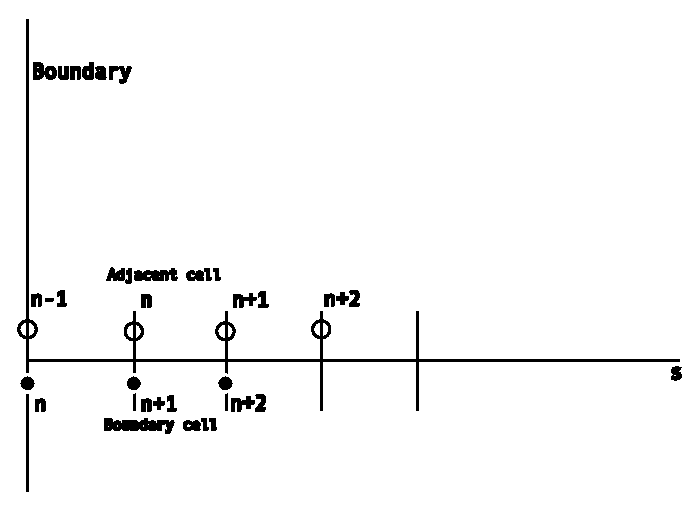
\includegraphics[width=0.7\textwidth]{Boundarydiff.eps}
\caption{Schematic showing the cells of intest in the differencing scheme when considering the boundary cell (Hollow circles) and the adjacent cell (Filled circles).  The figure shows the left hand boundary, for right hand simply reflect in the y direction}
\label{boundarydiffs}
\end{center}
\end{figure}

When the advective velocity is negative the opposite is true and the right hand boundary is differenced as follows,

\begin{eqnarray}
\mbox{Boundary cell} &-& \mbox{Second order scheme} - \frac{\partial f}{\partial s} = \frac{\frac{3}{2}f_{n} - 2f_{n-1} +\frac{1}{2}f_{n-2}}{ds}\nonumber\\
\mbox{Adjacent cell} &-& \mbox{Third order} - \frac{\partial f}{\partial s} = \frac{\frac{1}{3}f_{n+1} +\frac{1}{2}f_{n} - f_{n-1} + \frac{1}{6}f_{n-2}}{ds}\nonumber
\end{eqnarray}

\begin{figure}
\begin{center}
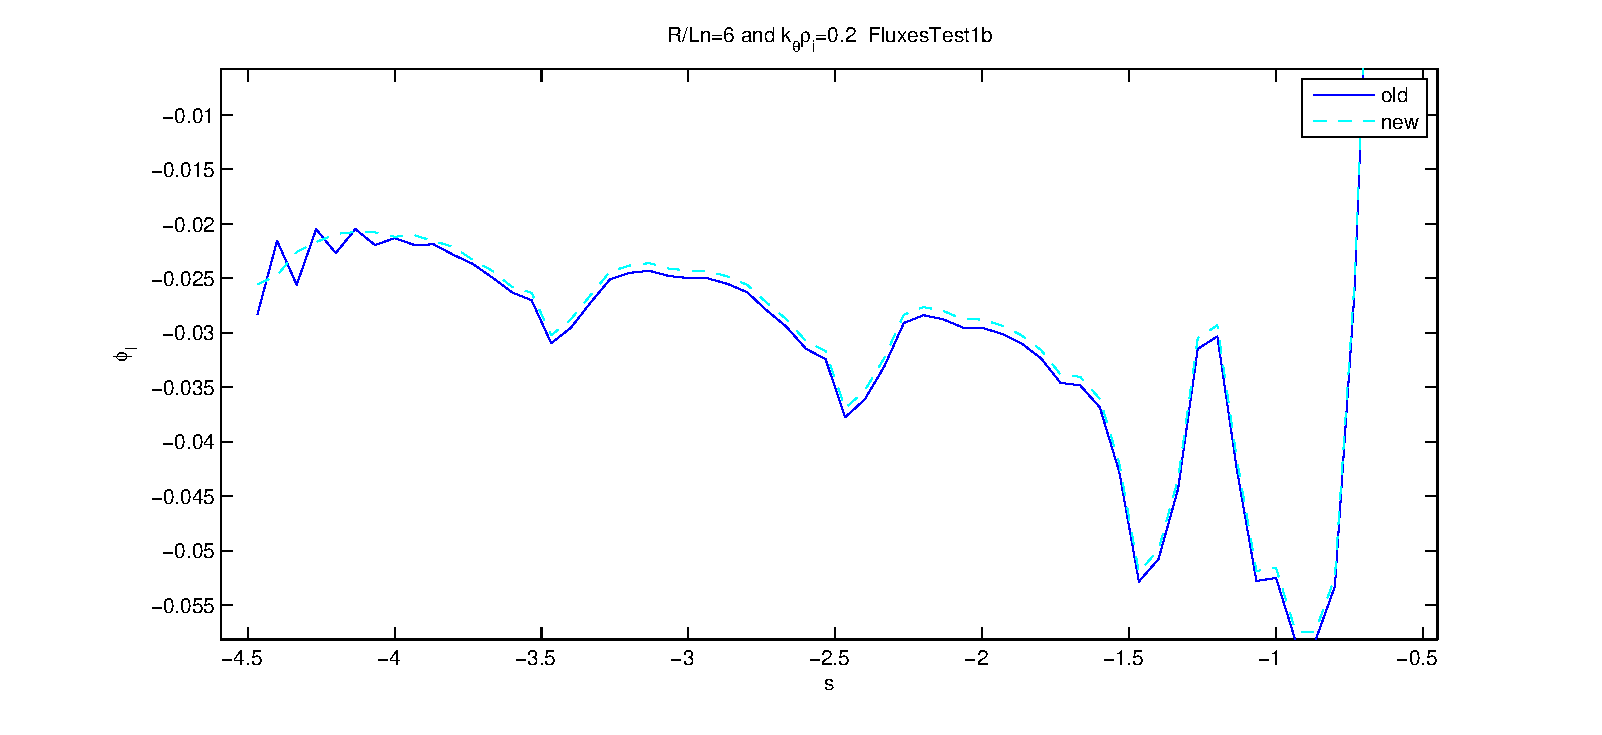
\includegraphics[width=0.95\textwidth]{fluxcomp.eps}
\caption{Figure showing the effect of the new open boundary conditions at the boundary. The new boundary has reduced cell to cell fluctuations giving a smoother solution.}
\label{fluxcomp}
\end{center}
\end{figure}

\noindent
Currently there is no dissipation (Diffusion/super-diffusion) within this scheme.


When using the second order scheme is used only special consideration is needed for the boundary cell.  Depending on the direction of the advective velocity a first order backwinded scheme is used at the boundary while the opposite uses the second order central differenced scheme with a ghost cell whose value is determined by the \textbf{parallel\_boundary\_conditions} parameter. 

The effect of these new open boundary conditions is to remove the need for ghost cells in the differencing scheme while maintaining a high order scheme. It has reduced the amplitude of cell to cell fluctuations refelecting off the boundary (See figure \ref{fluxcomp}), which in turn, has reduced the need for adding artificial dissipation to the system to damp away these modes.  The dissipation, however, can not be wholly turned off in non-linear runs.  Note also that the dealiasing in nonlinear runs also has some dissipative effect in the perpendicular spatial directions.

\section{Parallel velocity grid - Trapping condition}%Added by Will 29/6/2008
\index{trapping condition}
By contorting the velocity grid to conform to the electron trapping condition we are able to remove terms that involve derivatives in the parallel velocity direction.  This greatly speeds up linear run computation times but more significantly removes the need for numerical diffusion in the parallel velocity direction and lastly, provides resolution in the required areas.

This option is turned on by setting \textbf{vp\_trap} $= 0$ in the \textbf{CONTROL} section of the input deck.  A further parameter is needed in the same section which is named \textbf{n\_trapped} which is the number of grid points within the trapped region of the velocity grid.

One point of note is in the current implementation of the trapping condition the number of cells in the s direction and the number of points in the parallel velocity direction add certain constrictions to the number of points that can be placed within the trapped region.

Firstly, for ease of differencing the bounce points of a specific $v_{\parallel 0}$ (The velocity on the low-field side) must occur exactly half way between two grid-cells, thus the number of grid cells in the s direction restrict both the number and initial values of $v_{\parallel}$.  The maximum number of bounce points available is given by $ns/2 - 1$.  The value of ntrapped must be less than or equal to this.  If less is chosen then the code will select which points to use determined by the spacing between points (The closer to the boundary, the closer the bounce points become), the algorithm will iterate over the points, sequentially removing points until ntrapped are left.  ntrapped must also be less than nvpar.  Outside the trapping region the points are uniformly placed, the spacing is determined by the number nvpar $- 2\times$n\_trapped.

\begin{figure}[here!]
\begin{center}
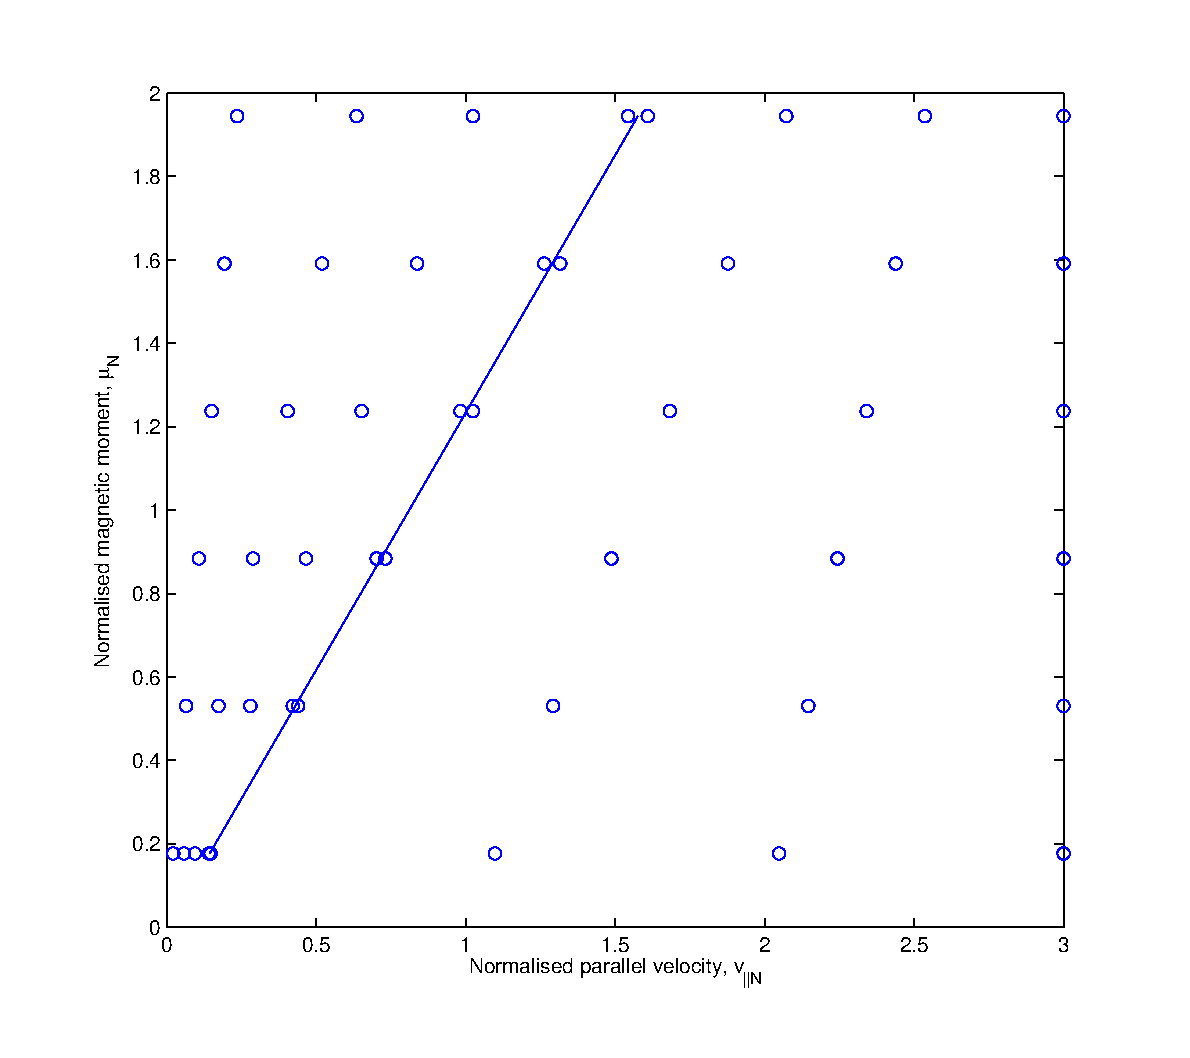
\includegraphics[width=0.7\textwidth]{traplowfield.eps}
\caption{Figure of parallel velocity grid points as given by the trapping condition, the line corresponds to the trapped/untrapped boundary $v_{||0} = \sqrt{2\mu(B_{max}-B_{min})}$.  In the above data, N\_vpar\_grid $= 16$ (only one half of the grid is shown as it is symmetric),n\_trapped $= 4$ and $\mu = 6$. It must be noted that the total number of points within the trapped region (full grid) is $2\times$n\_trapped.}
\label{lowfieldsidetrap}
\end{center}
\end{figure}

This algorithm gives the grid at the low field side (For an example see figure \ref{lowfieldsidetrap}), this is then propagated around the torus by the equation,

\begin{equation}
v_{\parallel N} = \sqrt{v_{\parallel 0 N}^{2} + 2\mu_{N}(B - B_{0})}
\end{equation}
\noindent
Where $B_{0}$ is the magnetic field at the low field side.  When a bounce point is reached, the velocity becomes zero, all points after this along s are essentially set to zero and are ignored in the differencing.  The grid is also symmetric around $v_{\parallel}=0$.


Rules that must be followed, otherwise the code will throw you out,
\begin{itemize}
\item The value of ntrapped must be less than N\_vpar\_grid/2
\item ntrapped must also be less than or equal to ns/2$-1$
\item For optimal convergence $2\times$n\_trapped must be roughly half of nvpar for more information on convergence properties see figure \ref{}.
\end{itemize}

%WAH: \begin{figure}
%WAH: \begin{center}
%WAH: \includegraphics[width=0.9\textwidth]{Killer3.eps}
%WAH: \caption{The absolute error in growth rates as a function of the mean parallel velocity element.}
%WAH: \label{converge}
%WAH: \end{center}
%WAH: \end{figure}

\printindex

\end{document}
